\chapter[The Compressibility of Saturn's Magnetosphere]{The Compressibility of Saturn's Magnetosphere in Response to Internal and External Influences}
\label{chap:compress}

In this chapter, we present the results  of an investigation into the compressibility of Saturn's dayside magnetosphere in response to changing internal  and external influences. These influences include the global hot plasma content in the magnetosphere, which inflates the magnetosphere and  enhances the ring current activity, and the external solar wind dynamic pressure $D_\mathrm{P}$, which controls the overall system size. Previous empirical studies assumed that Saturn's magnetopause stand-off distance varies as $D_\mathrm{P}^{-1/\alpha}$, and measured a constant compressibility parameter $\alpha$ corresponding to behaviour intermediate between a vacuum dipole appropriate for Earth ($\alpha \approx 6$), and a more easily compressible case appropriate for Jupiter ($\alpha \approx 4$). In this chapter we employ the 2-D force-balance model of Saturn's magnetodisc from \citet{achilleos2010a}, described in Section~\ref{intro:sec:forcebalancemodel} of this thesis, to investigate relationship in response to changes in $D_\mathrm{P}$ and global hot plasma content. For hot plasma levels compatible with Saturn observations, we model the magnetosphere at a range of stand-off distances and estimate the corresponding $D_\mathrm{P}$ values by assuming pressure balance across the magnetopause boundary. We find that for `average' hot plasma levels, our estimates of $\alpha$ are not constant with $D_\mathrm{P}$, but vary from ${\sim}4.8$ for high $D_\mathrm{P}$ conditions, when the magnetosphere is compressed (${\leq}\SI{25}{R_S}$), to ${\sim}3.5$ for low $D_\mathrm{P}$ conditions. This corresponds to the magnetosphere becoming more easily compressible as it expands. We also find that enhanced global hot plasma content increases magnetospheric compressibility even at fixed $D_\mathrm{P}$, with $\alpha$ estimates ranging from ${\sim}5.4$ to ${\sim}3.3$ across the range of our parameterised hot plasma content. We suggest that this behaviour is predominantly driven by reconfiguration of the magnetospheric magnetic field into a more disc-like structure under such conditions. In a broader context, the compressibility of the magnetopause reveals information about global stress balance in the magnetosphere, which we discuss in this chapter. The contents of this chapter are heavily based on the published study by \citet{sorba2017}.

\section{Introduction}\label{compress:sec:intro}
We discussed in Chapter~\ref{chap:intro} how in a steady-state system, the shape and size of a planetary magnetopause is determined by pressure balance across the boundary, between the internal magnetic and plasma pressures of the magnetosphere, and the pressure associated with the shocked solar wind plasma of the magnetosheath. The pressure exerted by the solar wind is principally due to the component of the dynamic pressure $D_\mathrm{P}$ that is normal to the magnetopause surface, where $D_\mathrm{P}$ is defined as $\rho_mu_\mathrm{SW}^2$ ($\rho_m$ denotes solar wind mass density and $u_\mathrm{SW}$ is the velocity). The dayside magnetosphere is compressed when the upstream dynamic pressure increases, and inflates when the dynamic pressure drops. The magnetopause is therefore in constant motion, with a velocity of order {\SI{10}{km s^{-1}}} for Earth's magnetopause {\citep{berchem1982}}, and {\SI{100}{km s^{-1}}} for Saturn's {\citep{masters2011}}. However to first order, its location can be approximated by assuming Newtonian pressure balance across the surface. 

A useful proxy of the overall size scale of a magnetosphere is the `stand-off distance', $R_\mathrm{MP}$. This is the location of the magnetopause boundary measured from the planet center along the planet-Sun line, i.e. the sub-solar nose of the magnetosphere. At this point, the solar wind flow direction is perpendicular to the magnetopause surface, and so the pressure balance relation defined in Equation~\ref{intro:eq:pbalance2} simplifies to
\begin{equation}\label{compress:eq:pbalance}
\frac{B_{\mathrm{MS}}^2}{2\mu_0} + P_{\mathrm{MS}} = kD_\mathrm{P}.
\end{equation}
$B_\mathrm{MS}$ is the magnetic field strength just inside the magnetopause boundary, which comprises the internal planetary field and other sources, such as the field associated with a magnetospheric ring current. $P_{\mathrm{MS}}$ is the total plasma pressure just inside the magnetopause boundary, the relative significance of which varies greatly between planets, as discussed in Section~\ref{intro:sec:comparativemagnetospheres}. $k$ is a positive constant $\leq1$ to account for the diversion of solar wind flow around the magnetospheric obstacle, and depends on the ratio of specific heats $\gamma$ in the solar wind, and the upstream sonic Mach number $M$. 

A key source of pressure inside all planetary magnetospheres is the magnetic pressure $P_\mathrm{B}=B_\mathrm{MS}^2/2\mu_0$. We can therefore estimate the value of $R_\mathrm{MP}$ to first order, by finding the radial distance from the planet center $r$ at which the magnetic pressure is  balanced by the solar wind dynamic pressure. If we make the assumption $B \propto r^{-\chi}$, such that the magnetic pressure $P_\mathrm{B} \propto r^{-2\chi}$, we can then write
\begin{equation}\label{compress:eq:key}
R_\mathrm{MP}=a_1D_\mathrm{P}^{-1/\alpha}
\end{equation}
where $a_1$ is a constant that determines the size scale of the system and $\alpha$ is the `compressibility parameter', equal to $2\chi$. This relationship is used to model the overall size of the magnetosphere in studies of the planets Earth, Jupiter and Saturn, as described in detail below. 

For a vacuum dipole magnetic field $\chi=3$, giving $\alpha=6$. This is broadly consistent with observations of Earth's magnetosphere, such as \citet{shue1997}. However in contrast to the terrestrial system, Saturn's magnetosphere has significant internal plasma sources; a cold population originating from the icy moon Enceladus \citep[e.g.][]{dougherty2006,tokar2006}, and a hotter population that is more variable with radial distance and over time \citep[e.g.][]{sergis2009}. Saturn also rotates more rapidly  than the Earth, with a ${\sim}\SI{10.7}{hour}$ period \citep{desch1981}. As discussed in detail in Sections~\ref{intro:sec:comparativemagnetospheres} and \ref{intro:sec:saturn}, these conditions causes Saturn's magnetosphere to form a more `disc-like' configuration, with magnetic field lines `stretched' radially outwards near the equatorial plane, supported by an azimuthal ring current. This magnetic field configuration affects the compressibility parameter $\alpha$, since for a disc-like magnetic field, $B$ varies more slowly with radial distance in the outer magnetosphere than for a dipole. This can be seen in Figure~\ref{compress:fig:magdata}, which shows the total magnetic field strength measured by the \textit{Cassini} MAG instrument in Saturn's dayside magnetosphere, taken from 3 equatorial orbits during Saturn equinox (Revs $120{\--}122$, 23~October to 17~December~2009). In the inner and middle magnetosphere the data appear to be well approximated by the relationship $B \propto r^{-3}$. However in the outer magnetosphere ($r \gtrsim \SI{15}{R_S}$), where the magnetic field associated with the ring current is more significant compared to the internal dipole magnetic field, the data appear better approximated on average by a relationship $B \propto r^{-2}$, i.e. a lower value of $\chi$, and therefore a lower value of $\alpha$. This means that with a magnetodisc magnetic field structure, the magnetosphere size is expected to be more sensitive to changes in solar wind pressure than for a dipole case, as the index $-1/\alpha$ in equation~\ref{compress:eq:key} is greater.

\begin{figure}
\centering
\noindent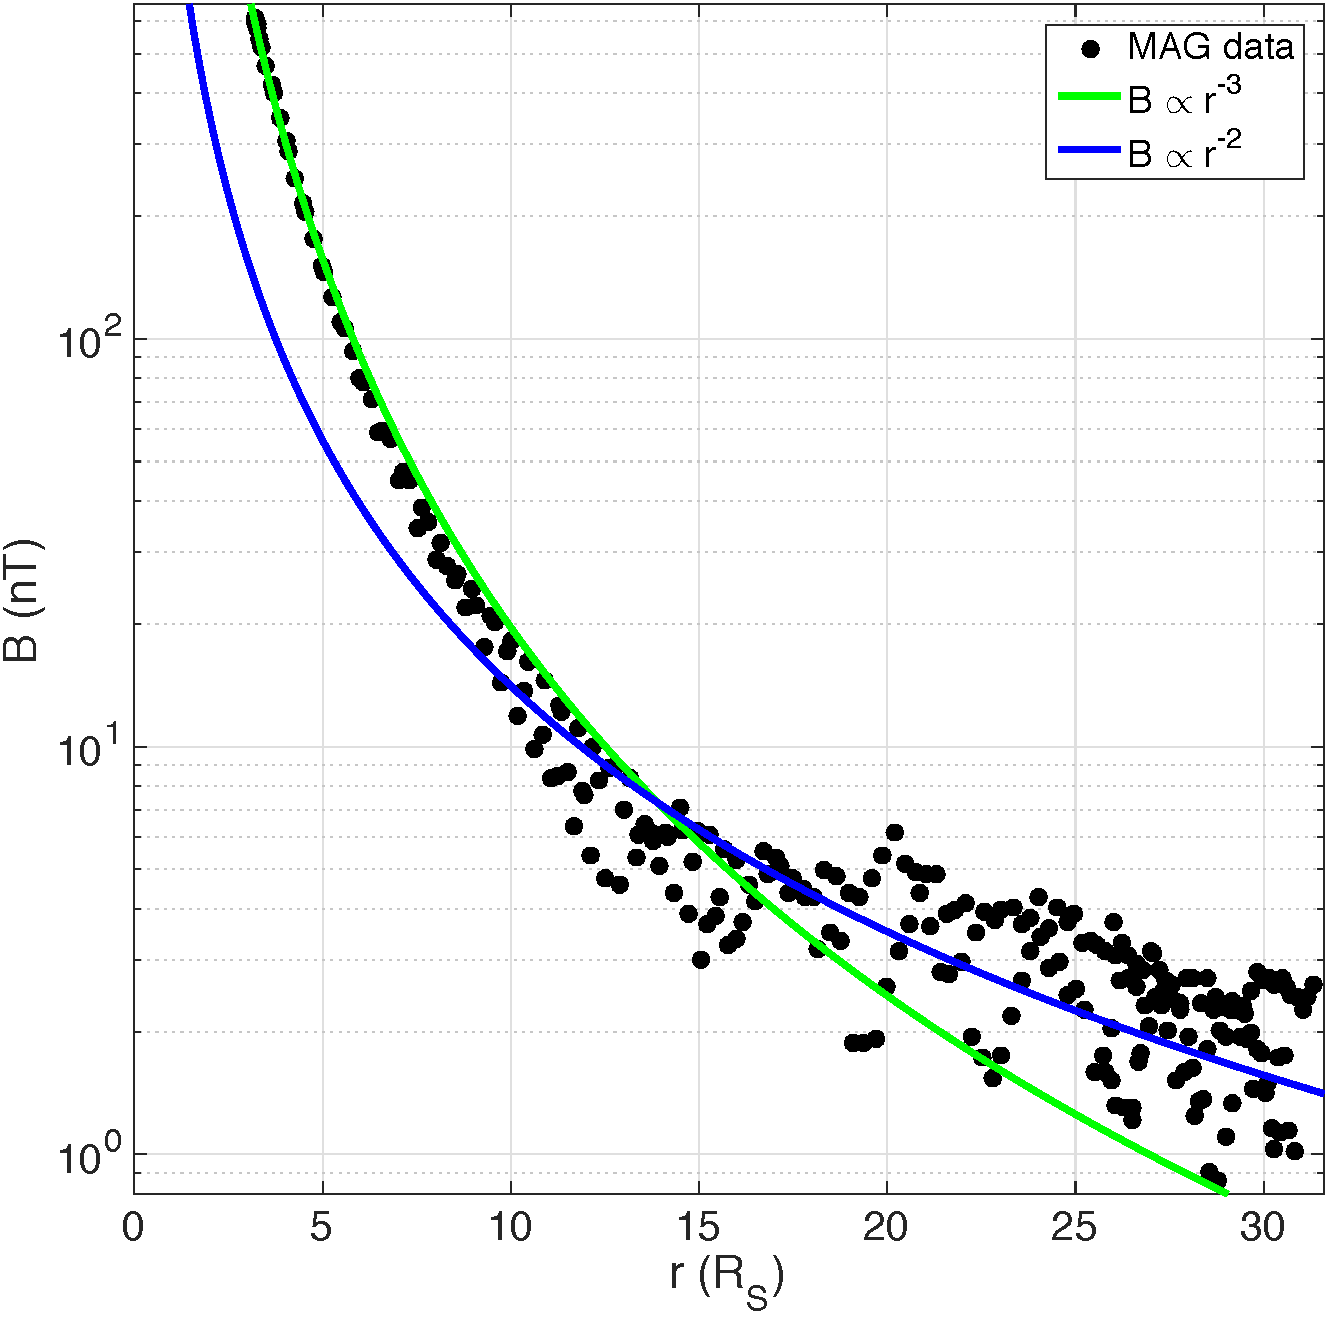
\includegraphics[width=0.6\textwidth]{compress/magdata.pdf}
\caption[Equatorial magnetic field data from \textit{Cassini} MAG.]{Total magnetic field strength $B$ against radial distance from planet center. Black circles are from \textit{Cassini} MAG data, measured on Saturn's dayside, taken from 3 equatorial orbits during Saturn equinox (Revs $120{\--}122$, 23~October to 17~December~2009). Example power law curves shown in green and blue for reference.}
\label{compress:fig:magdata}
\end{figure}

In Saturn's middle and outer magnetosphere, the  hot  ($>\SI{3}{keV}$) plasma population contributes more to the total plasma pressure than the colder equatorial plasma,  and values of plasma $\beta$ in the range ${\sim}2{\--}5$ have been observed  for this population in this region \citep{sergis2010}. This means that under some conditions the hot plasma population may control compressibility directly. The derivation of equation (\ref{compress:eq:key}) assumes the solar wind dynamic pressure is directly balanced by the magnetic pressure inside the magnetosphere; however, for $\beta > 1$ at the magnetopause boundary, the hot plasma pressure inside the magnetosphere is also significant in controlling pressure balance. Therefore $\alpha$ will be partially determined by how the hot plasma pressure $P_\mathrm{H}$ varies with radial distance (via the same arguments as laid out for equation (\ref{compress:eq:key}) above). \citet{gold1959} used the concept of magnetic flux tubes of plasma expanding isothermally to explain that, in a dipolar magnetic field, one would expect the hot plasma pressure to fall with radial distance according to $P_\mathrm{H} \propto r^{-4}$. We would thus expect $\alpha = 4$ for a fictitious magnetosphere where compressibility is dominantly controlled by a hot plasma population embedded in a dipole magnetic field, and a value even smaller for a magnetic field that varied more slowly than $r^{-3}$. We expand on this in Section~\ref{compress:sec:hotplasma}.

Jupiter's magnetosphere also has a significant internal plasma population, due to mass loading from the volcanic moon Io; the observed plasma $\beta$ associated with this population reaches 100 at \SI{45}{R_J} \citep{mauk2004}. The associated centrifugal force is also greater than the Saturnian parallel, mainly due to the larger overall size scale of Jupiter's magnetosphere, as discussed in Section~\ref{intro:sec:comparativemagnetospheres}. These conditions produce a more substantial disc-like magnetic field configuration at Jupiter, which significantly affects the magnetospheric compressibility; $\alpha$ has been measured empirically for this system as between ${\sim}4$ and ${\sim}5$ \citep{huddleston1998, joy2002, alexeev2005}. However these estimates are based on limited spacecraft observations and hence have large uncertainties associated with them.

Saturn's magnetosphere would therefore be expected to show compressibility behaviour that is intermediate between that of Jupiter ($\alpha \approx 4$) and the Earth ($\alpha \approx 6$). The inter-related factors of magnetic field structure, centrifugal force and plasma content that determine the overall stress balance may themselves show behaviour that varies with solar wind dynamic pressure (i.e. vary with size of the magnetosphere). It is therefore insightful to investigate Saturn's magnetospheric compressibility in response to changes in both external factors (the incident solar wind dynamic pressure) and internal factors (hot plasma content) in tandem.

\subsection{Models of Saturn's Magnetopause}\label{compress:sec:prevstudies}
\begin{table}
\caption[Estimates of magnetopause model parameters from previous studies.]{Estimates of magnetopause model parameters from previous studies.}\label{compress:table:prevstudies}
\centering
\begin{tabular}{c c c c}
\hline
Study & Size Range $(\si{R_S})$ & $a_1$ & $\alpha$   \\
\hline
{\citet{slavin1985}} & $< 19$ &  & $\sim 6.1$ \\
{\citet{hansen2005}}   & $21 - 28 $ &  & $\sim 5.2$ \\
{\citet{arridge2006}} & $17-29$ & $9.7 \pm 1.0 $ & $4.3 \pm 0.4$   \\
{\citet{kanani2010}} & $17-29$ & $10.3 \pm 1.7 $ & $5.0 \pm 0.8$ \\
{\citet{pilkington2015}} & $14 - 40$ & $10.8 - 16.5$ & $5.5 \pm 0.2$ \\
\hline
\end{tabular}
\end{table}
Previous studies have mostly employed \textit{in situ} magnetopause crossing data to create empirical models of the size and shape of Saturn's magnetosphere under different solar wind pressure conditions, in order to make estimates of $\alpha$ and $a_1$. \citet{slavin1985} used \textit{Pioneer} 11 and \textit{Voyager} 1 and 2 plasma and magnetometer data and modelled the magnetopause surface as a conic section. \citet{arridge2006} applied the formalism first described in \citet{shue1997} for the terrestrial system to Saturn using \textit{Cassini} MAG data, estimating the upstream solar wind pressure by assuming pressure balance with the magnetic pressure of the magnetosphere just inside the magnetopause. This model was then augmented by \citet{kanani2010} who used \textit{Cassini} plasma data in order to include thermal plasma pressure, as well as magnetic pressure, inside the magnetopause. Further improvements to the treatment of internal plasma pressure sources, and an extension of the crossing data set, were then made by \citet{pilkington2015}. Previous to these \textit{Cassini}-based studies, \citet{hansen2005} used a 3-D global magnetohydrodynamic simulation of Saturn's magnetosphere for the time period of \textit{Cassini}'s initial approach in order to investigate $\alpha$. The relevant parameters calculated in each study are shown in Table~\ref{compress:table:prevstudies}, where parameters relate to equation~\ref{compress:eq:key} with $R_\mathrm{MP}$ in units of $\si{R_S}$ and $D_{P}$ in nanopascals (\si{nPa}). In the study by \citet{pilkington2015}, they explain that their extended \textit{Cassini} data set includes more variable and high-$\beta$ crossings than previous studies. A k-means clustering algorithm was used to separate the crossing data set into three groups organized by local plasma $\beta$; while the estimates of $\alpha$ agreed in each group within the uncertainties, the estimates of $a_1$ did not, and showed a trend of increasing with larger average $\beta$, from ${\sim}10.8$ to ${\sim}16.5$.

The estimates of $a_1$ by \citet{arridge2006} and \citet{kanani2010} agree within the quoted uncertainties. In addition, in \citet{pilkington2015}, in order to account for the influence of local plasma $\beta$ on $a_1$, these authors repeat their analysis with a modification to equation~\ref{compress:eq:key} such that $D_\mathrm{P}$ is replaced by $D_\mathrm{P}/(1+\beta)$. With this adaptation, \citet{pilkington2015} measured $a_1 = 10.5 \pm 0.2$, which is consistent with previous results shown in Table~\ref{compress:table:prevstudies}. The estimates of $\alpha$ for each study agree at least within 2$\sigma$ uncertainty level, where appropriate, and in general are consistent with the picture of a magnetosphere that behaves intermediately between the rigid Earth case and the more compressible Jupiter case. However the role of the global hot plasma content in controlling magnetospheric compressibility is still not fully understood.

The current lack of multi-point simultaneous observations in Saturn's magnetosphere mean that the use of \textit{in situ} data is inherently limited, as the large scale structure of the magnetosphere at the exact time corresponding to one magnetopause crossing cannot be readily obtained. This makes it difficult to interpret the global physical processes that are controlling the compressibility behaviour. Instead empirical studies, such as those referred to above, provide an `average' picture of the magnetopause morphology over varying internal and external conditions. In addition, the empirical studies discussed must assume that the magnetopause is in dynamical equilibrium at the time of crossing observations (i.e. it is not accelerating) in order to estimate the solar wind pressure via Newtonian pressure balance, which is almost never the case at Saturn \cite[e.g.][]{dougherty2005,masters2011,pilkington2015}.

In this study we adopt a more theoretical approach, in order to complement these previous observational studies. The 2-D axisymmetric force-balance model of Saturn's dayside magnetosphere, first presented by \citet{achilleos2010a} and described in Chapter~\ref{chap:intro}, is used to investigate magnetospheric compressibility. This model can be calculated at a chosen range of magnetopause radii. The corresponding estimated upstream solar wind pressure can be readily obtained using calculated plasma and magnetic field information just inside the magnetopause boundary and assuming pressure balance across the magnetopause, which is static in this model. These theoretical estimates of $D_\mathrm{P}$ can then be used to make estimates of $\alpha$ and $a_1$. In addition, \citet{achilleos2010a} referred to a `hot plasma index' in the model, with which the hot plasma content in the magnetosphere can be parameterised. We revisit this concept herein, in order to investigate the influence of the global hot plasma population on magnetospheric compressibility.

\section{Method}\label{compress:sec:method}
\subsection{Magnetodisc Model Calculations}\label{compress:sec:model}
In this study we use the UCL/AGA model for Saturn's magnetodisc originally set out in \citet{achilleos2010a}, and described in detail in Section~\ref{intro:sec:forcebalancemodel} of this thesis. As a reminder, the model is axisymmetric about the planetary dipole/rotation axis, which are assumed to be aligned, and is constructed based on the assumption of force balance in the rotating plasma of the magnetosphere such that 
\begin{equation*}\label{compress:eq:forcebalance}
\boldsymbol{J} \times \boldsymbol{B} = \nabla P - nm_i\omega^2\rho\boldsymbol{\hat{\rho}} \tag{\ref{intro:eq:forcebalance} revisited}
\end{equation*}
where $\boldsymbol{J}$ is the current density, $\boldsymbol{B}$ is the magnetic field vector and $\rho$ is cylindrical radial distance from the axis, with $\boldsymbol{\hat{\rho}}$ its unit vector. The plasma properties are isotropic pressure $P$, ion number density $n$, mean ion mass $m_i$ and angular velocity $\omega$. The model assumes the magnetospheric plasma comprises a cold population with pressure $P_\mathrm{C}$, confined towards the rotational equatorial plane due to the centrifugal force exerted on it, and a hot population with associated plasma pressure $P_\mathrm{H}$ constant along magnetic field lines. 

For the cold plasma population, the pressure is constrained by equatorial radial profiles of plasma properties, obtained from studies using the \textit{Cassini} CAPS and MIMI instruments, as summarised in \citet{achilleos2010a,achilleos2010b}. For  the hot plasma population, the pressure $P_\mathrm{H}$ may be completely characterized by a particular equatorial plasma pressure $P_\mathrm{H0}$, and flux tube volume $V$ per unit of magnetic flux, where
\begin{equation}\label{compress:eq:ftv}
V = \int_{0}^{s_{B}} ds/B, \tag{\ref{intro:eq:ftv} revisited}
\end{equation}
and $ds$ is an element of arc length along the magnetic field line. The integral limits represent measurement along a field line of total length $s_B$ between the southern and northern ionospheric footprints at $\SI{1}{R_S}$. The flux tube volume is therefore dependent on both the shape of magnetic field lines, via $ds$, and the strength of the field, via $B$. 

\citet{achilleos2010a} combined quantile fits of equatorial profiles of equatorial hot plasma pressure \citet{sergis2007} with a radial profile of $V$ obtained from an empirical magnetic field model \citep{bunce2007} in order to show a picture of a highly variable hot plasma population, that follows neither adiabatic ($P_\mathrm{H0}V^{5/3} =$ constant) nor isothermal ($P_\mathrm{H0}V =$ constant) transport behaviour. In light of these observations, the original \citet{achilleos2010a} model simply parameterised the global hot plasma content by a single `hot plasma index' $K_\mathrm{H}$, where $ K_\mathrm{H}= P_\mathrm{H0}V$ is constant beyond $\SI{8}{R_S}$, and $P_\mathrm{H0}$ decreases linearly to zero inside that distance. A similar parameterisation, though with different values of the constants, was made in \citet{caudal1986}, who argued that for the Jovian system, under the expected conditions of rapid radial diffusion, the hot plasma would be transported isothermally. Parameterising the hot plasma content in this way provides the flexibility to very simply characterize the level of ring current activity in the model, and thus investigate the effect of the hot plasma content on magnetospheric compressibility. We recognize that more detailed studies of hot plasma dynamics may require investigation of different parameterisations in the future. In particular, a more physically realistic hot plasma profile was developed in \citet{achilleos2010b}, however the use of such a profile does not affect the basic conclusions of this study.

In this study a value of $K_\mathrm{H}=\SI{1e6}{Pa m T^{-1}}$ was initially adopted to parameterise the ring current activity in the magnetosphere, representing broadly `average' conditions, corresponding to the median quantile fit of the hot plasma pressure from \citet{sergis2007}. The magnetodisc model was then calculated at 30 different magnetopause radii $R_\mathrm{MP}$, equally spaced over a range of $14{\--}\SI{40}{R_S}$, in order to match the range in this parameter observed in the data set presented by \citet{pilkington2015}. For each calculation, the corresponding solar wind dynamic pressure incident on the magnetopause nose was estimated from model magnetospheric parameters by assuming pressure balance across the model magnetopause boundary. Specifically, we used the relationship given in equation~\ref{compress:eq:forcebalance}, with $P_{\mathrm{MS}}=P_\mathrm{H}+P_\mathrm{C}$, extracting values for $B_\mathrm{MS}$, $P_\mathrm{H}$ and $P_\mathrm{C}$ from the model just inside the magnetopause boundary at the equator. For $k$, we used a value of 0.881, as this is appropriate for high ($\gtrsim 8$) Mach number flow with $\gamma = 5/3$  \citep{spreiter1966}, which is valid for the solar wind at Saturn's orbit \cite[e.g.][]{slavin1985,achilleos2006}. However as it is of order unity it does not significantly affect our estimates of $D_\mathrm{P}$ or the conclusions of this study. This value of $k$ is also used in the previous studies discussed in Section~\ref{compress:sec:prevstudies}.

A profile of $R_\mathrm{MP}$ versus $D_\mathrm{P}$ for a given $K_\mathrm{H}$ value was then constructed in order to estimate the model compressibility parameter $\alpha$. The value of $K_\mathrm{H}$ in the model was then varied linearly over the range $10^5{\--}10^7~\si{\pascal\meter\per\tesla}$, in accordance with aforementioned  observations, and the effect on magnetospheric compressibility was investigated. 


\subsection{Fitting Procedure and Uncertainty Estimation}
We made estimates of the compressibility parameter $\alpha$ for each profile of $R_\mathrm{MP}$ and $D_\mathrm{P}$ simulated data points using linear least squares regression analysis as follows. If we have a set of $n$ data points $\{x_i,y_i\}$ that we have reason to believe are linearly dependent, we can attempt to find a `best fit line' to describe this relationship, $\hat{y}(x) = mx + b$. In our study, this corresponds to the logarithm of equation~\ref{compress:eq:key},
\begin{equation}
\log{R_\mathrm{MP}}{=}-1/{\alpha}\log {D_\mathrm{P}}+\log{a_1},
\end{equation}
such that $\hat{y} = \log{R_\mathrm{MP}}$, $x =\log{D_\mathrm{P}}$, $ m = -1/\alpha$ and $b = \log{a_1}$. We can then obtain estimates of parameters $a_1$ and $\alpha$ by fitting the logarithms of our simulated data set, $\{x_i=\log{D_\mathrm{P}}$, $y_i=\log{R_\mathrm{MP}}\}$ with a best fit line, and estimating $m$ and $b$.

In order to obtain estimates of the parameters $m$ and $b$, we minimize the sum of the squares of the residuals between the data and the best fit line points,
\begin{equation}
SS = \sum\limits_{i=1}^{n}(y_i-\hat{y_i})^2,
\end{equation}
with respect to $m$ and $b$. This yields the solutions
\begin{align}
 m  &=  \frac{\sum(x_i-\bar{x})(y_i-\bar{y})}{\sum(x_i-\bar{x})^2}  \nonumber\\ 
 b & =   \bar{y} - m\bar{x} 
\end{align}
where $\bar{x}$ denotes the mean of all $x_i$, and similarly for $\bar{y}$, and all summations are calculated over all $n$ data points. This technique assumes the errors associated with the data are uniform such that all $\{x_i,y_i\}$ are weighted equally, and is known as the ordinary least-squares solution. The approximate standard errors of the parameters, $s_m$ and $s_b$, are then given by
\begin{align}
s_m^2 = & \frac{\hat{\sigma}^2}{\sum(x_i-\bar{x})^2}\nonumber\\
\nonumber\\
s_b^2 = & \frac{\hat{\sigma}^2\sum x_i^2}{n\sum(x_i-\bar{x})^2}
\end{align}
where $\hat{\sigma}^2 = SS/(n-2)$ is the estimated variance in the simulated `measurements', and $(n-2)$ is the number of degrees of freedom. $s_m$ and $s_b$ are estimates of the changes in $m$ and $b$ that correspond to changes of order $\hat{\sigma}^2$ in $y_i$. These estimates require that the parameters $m$ and $b$ are uncorrelated, which is a valid assumption over ranges in magnetospheric size where both $m$ and $b$ are approximately constant. These results are derived from matrix relations that are generalized for fittings with greater than two parameters; more information can be found in \citet{yang2005}.

The corresponding errors in the parameters $a_1$ and $\alpha$ are then calculated using standard error propagation given the relationship between them and $m$ and $b$ respectively; for a variable $u = u(v)$, the error in $u$, $\sigma_u$, is given by
\begin{equation}
\left|\frac{du}{dv}\right|\sigma_v.
\end{equation} 

\section{Results and Discussion}\label{compress:sec:results}
\subsection{Magnetospheric Compressibility with `Average' Hot Plasma Conditions}
\begin{figure}
\centering
\noindent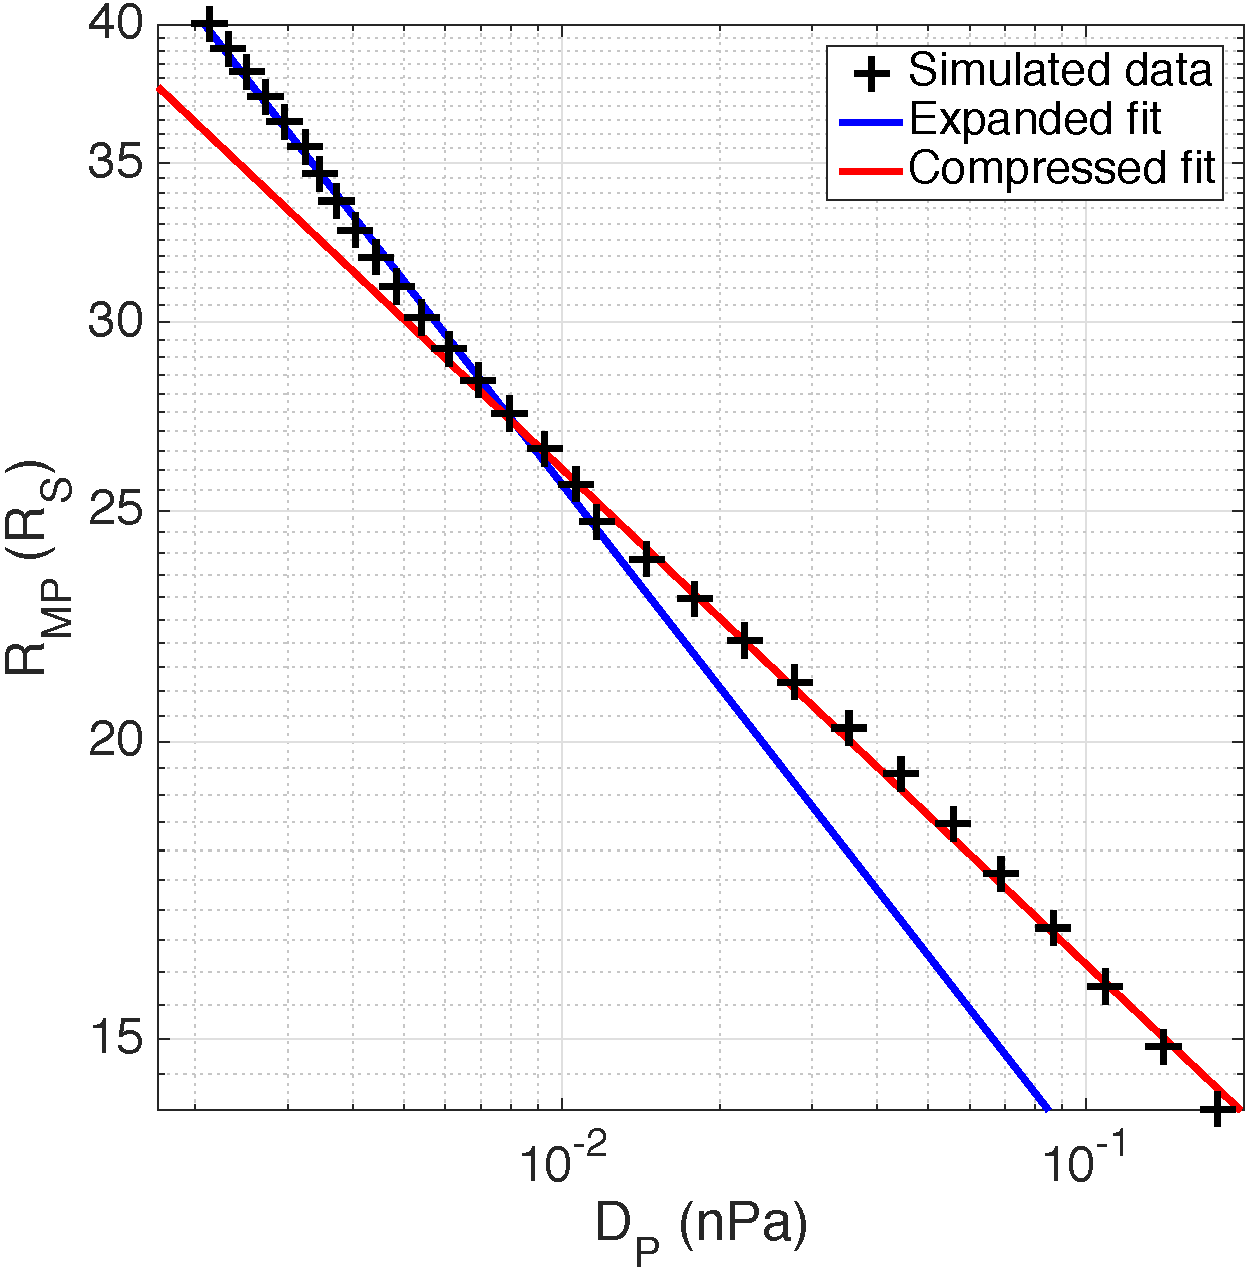
\includegraphics[width=0.6\textwidth]{compress/moneyplot.pdf}
\caption[Magnetopause radius versus solar wind dynamic pressure compressibility profile for `typical' hot plasma content $K_\mathrm{H}$.]{Magnetopause radius $R_\mathrm{MP}$ as a function of solar wind dynamic pressure $D_{P}$, on a logarithmic scale, for $K_\mathrm{H}=\SI{1e6}{\pascal\meter\per\tesla}$. Each black cross represents the result of one model calculation. The linear least squares regression line fitted to calculations with $R_\mathrm{MP} \leq \SI{25}{R_S}$ is shown in red, and for calculations with $R_\mathrm{MP} > \SI{25}{R_S}$ shown in blue.}
\label{compress:fig:money1}
\end{figure}
Figure~\ref{compress:fig:money1} shows the magnetopause radius $R_\mathrm{MP}$ for each model calculation as a function of the corresponding solar wind dynamic pressure, calculated as described in Section~\ref{compress:sec:method}, on a logarithmic scale, with $K_\mathrm{H}=\SI{1e6}{\pascal\meter\per\tesla}$. Linear least squares regression lines have been fitted to two regions of the data as described in the caption.

On such a plot, data that exactly obey equation (\ref{compress:eq:key}) with constant $a_1$ and $\alpha$ would follow a straight line with slope $-1/\alpha$ and y-intercept $a_1$. However it can clearly be seen that for this simulated `data set', neither $a_1$ nor $\alpha$ are constant with system size.
In particular, a distinct shift in behaviour can be identified at $R_\mathrm{MP} \approx \SI{25}{R_S}$. We therefore divided the simulated data set into two groups, $R_\mathrm{MP} \leq \SI{25}{R_S}$, which we shall refer to as the compressed regime, and $R_\mathrm{MP} > \SI{25}{R_S}$, which we shall refer to as the expanded regime. We then fit each data group with a linear least squares regression line separately, in order to make estimates of relevant parameters and investigate how they differ as the system expands. It should be noted that the value of $\SI{25}{R_S}$ in particular was selected by eye, and a value up to ${\sim}\SI{28}{R_S}$ could be chosen to divide the two regimes, and does not significantly affect our conclusions.

\begin{table}
\caption[Estimates of compressibility parameters for this study.]{Estimates of compressibility parameters calculated from the model outputs shown in Figure \ref{compress:fig:money1}.}\label{compress:table:money1}
\centering
\begin{tabular}{c c c c}
\hline
Regime & Size Range $(\si{R_S})$ & $a_1$ & $\alpha$   \\
\hline
Compressed & $14 - 25 $ & $10.0 \pm 0.1  $ & $4.80 \pm 0.09$ \\
Expanded & $25 - 40 $ & $7.0 \pm 0.2$ & $3.53 \pm 0.06$ \\
\hline
\end{tabular}
\end{table}
The estimates for $\alpha$ and $a_1$ with standard error uncertainties, for the two regimes, are shown in Table~\ref{compress:table:money1}. The full fitting procedure and calculation of uncertainties are described in the Appendix. It should be noted that such uncertainties should be taken as a guideline only. We do not suggest that the data exactly follow this underlying distribution, and have made this simplification to give an overall picture of the behaviour, given the limitations of our simulated data set. Real observational data would of course be subject to significant measurement errors, and the resulting parameter uncertainties would be higher than those we have calculated for our simulations.

For the compressed regime, the estimates of $a_1$ and $\alpha$ are broadly consistent with the previous results shown in Table~\ref{compress:table:prevstudies} at the 2$\sigma$ level, except the $\alpha$ estimate of \citet{pilkington2015}. For the expanded regime, the estimated values are both significantly smaller than those calculated in any previous studies. The value of $\alpha = 3.53$ in particular corresponds to the magnetosphere becoming more sensitive to changes in solar wind pressure as it expands, and in fact becoming marginally more compressible than the Jovian system, indicated by the value of $\alpha < 4$ (see discussion in Section~\ref{compress:sec:prevstudies}).This implies that under appropriate conditions, the compressibility behaviour of the Jovian magnetosphere may actually be an intermediate between Earth and Saturn. This is investigated in more detail later in Section \ref{compress:sec:jup}.

It was shown in \citet{achilleos2008}, who studied the long term behaviour of the size of Saturn's magnetosphere as measured by \textit{Cassini}, that the magnetopause radius is well described by a bimodal probability distribution, with local maxima at $22 \pm \SI{1.5}{R_S}$ and $27 \pm \SI{1.3}{R_S}$ (apparently distinct from the typical distributions of the solar wind dynamic pressure). In the earlier empirical studies, the magnetosphere is more often observed in a compressed regime, as shown by the observed ranges in Table~\ref{compress:table:prevstudies}, due to the more restricted data sets available for use in those studies, and the higher average solar activity at the time of observations \cite[e.g.][]{hathaway2015}. Thus the corresponding estimates of $a_1$ and $\alpha$ are likely to be weighted more towards values typical of such conditions. We also find that our parameter estimates are very sensitive to the choice of hot plasma index $K_\mathrm{H}$, which may be a cause of the discrepancy between our results and previous studies. We shall investigate this aspect in depth in the following sections, but first we will look at which components of the internal structure contribute most to the formation of this `knee' in compressibility behaviour at ${\sim}\SI{25}{R_S}$, as seen in Figure~\ref{compress:fig:money1}.

Figure~\ref{compress:fig:pcomps} shows the individual contributions from the hot, cold and magnetic pressure components to the total magnetospheric pressure just inside the model's magnetopause boundary. It can clearly be seen that the magnetic pressure, $P_\mathrm{B}=B^2/2\mu_0$, is the dominant component for all system sizes. Values of plasma $\beta$ have been extracted for the hot and cold plasma populations separately, and the hot plasma beta $\beta_\mathrm{H}$ and cold plasma beta $\beta_\mathrm{C}$ are both $\lesssim 0.7$ across all system sizes, while the total plasma $\beta$ of the collective plasma surpasses unity for the largest system sizes, where $R_\mathrm{MP} \gtrsim \SI{30}{R_S}$. The hot and cold pressure components are comparable for $R_\mathrm{MP} \gtrsim \SI{25}{R_S}$, below which the cold pressure dominates. 
\begin{figure}
\centering
\noindent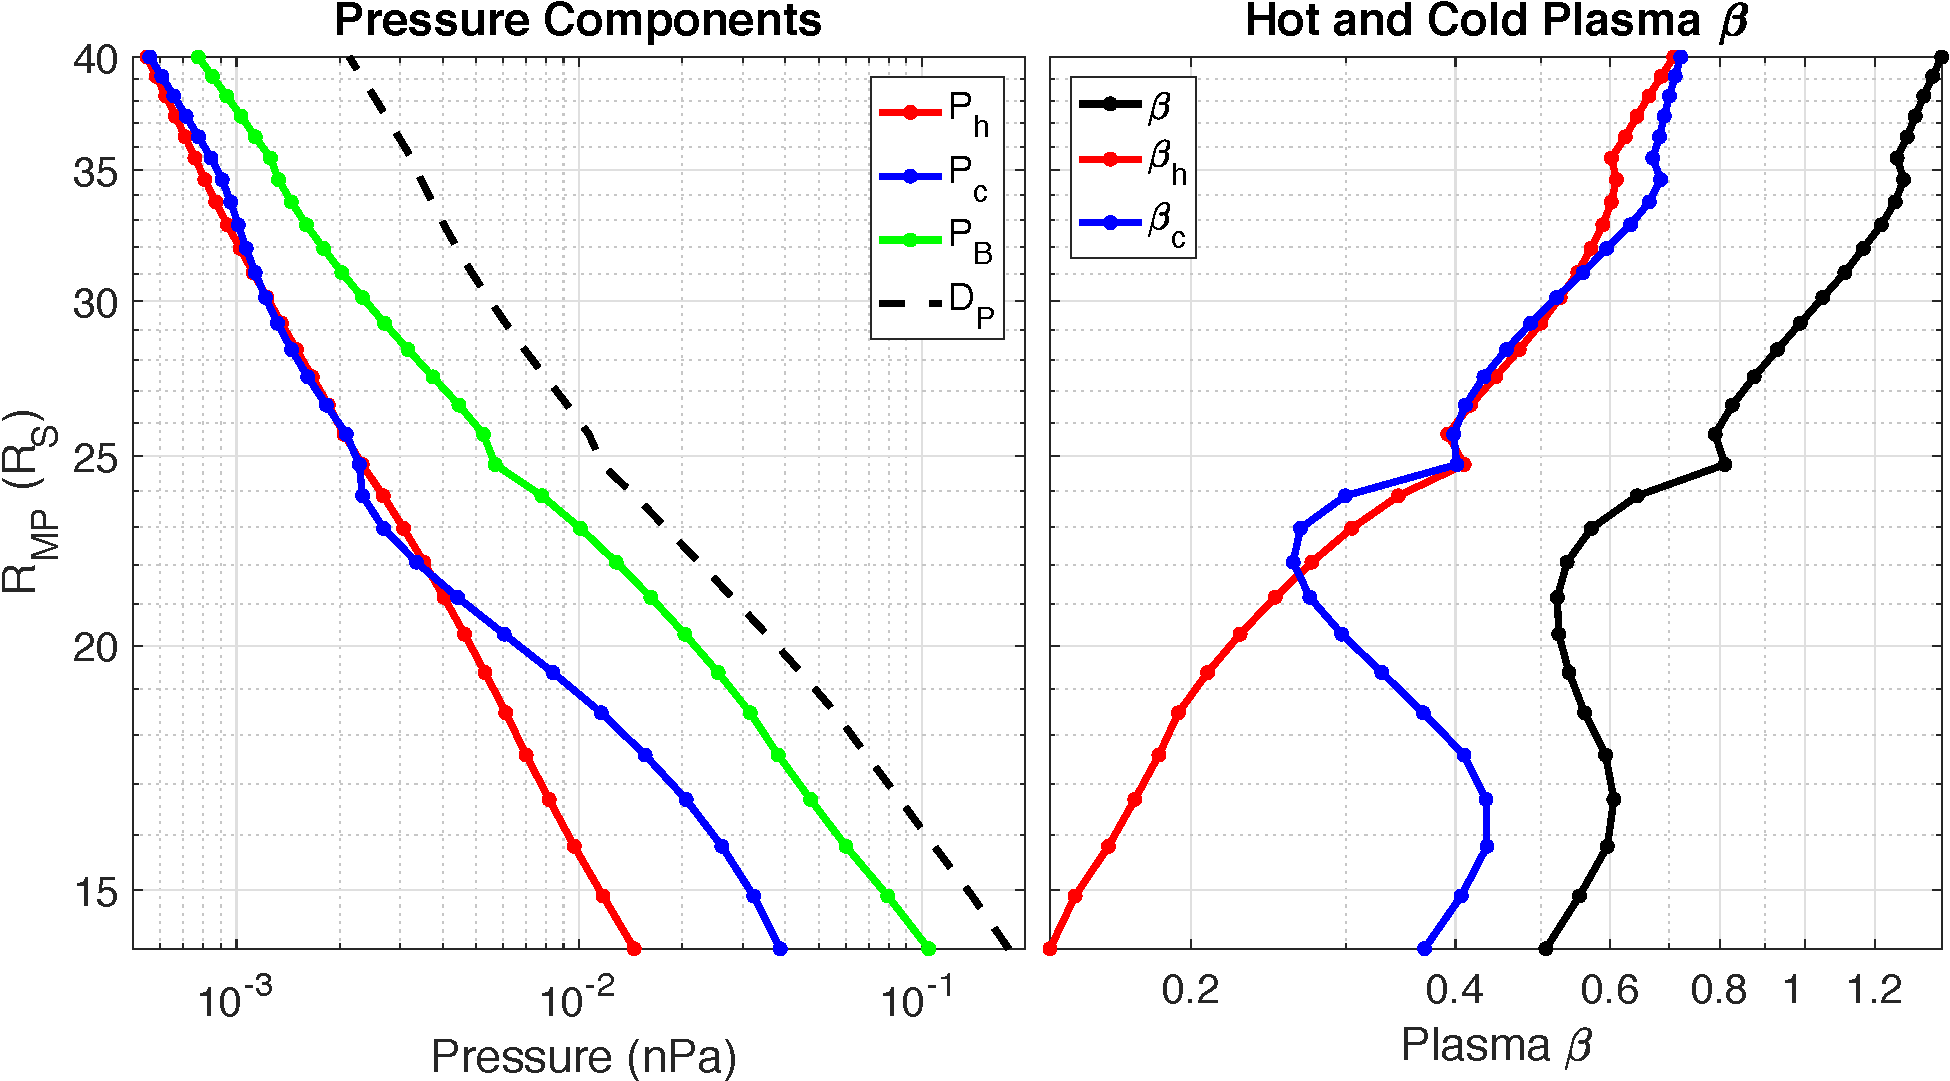
\includegraphics[width=\textwidth]{compress/pcomps.pdf}
\caption[Pressure components and plasma $\beta$ just inside the magnetopause boundary for typical $K_\mathrm{H}$.]{The individual contributions to the total magnetospheric pressure just inside the magnetopause boundary for different system sizes, corresponding to results in Figure~\ref{compress:fig:money1}. (left panel) The hot plasma, cold plasma and magnetic pressure components are shown in red, blue and green respectively, with the total pressure divided by $k=0.881$, i.e. the corresponding solar wind dynamic pressure, shown as a black dashed line for comparison. (right panel) The values of plasma $\beta$ just inside the magnetopause boundary for the collective plasma (black), and for each of the hot (red) and cold (blue) plasma populations separately.}
\label{compress:fig:pcomps}
\end{figure}
 
The magnetic pressure profile in particular appears to exhibit a change in gradient around $\SI{25}{R_S}$ similar to the solar wind pressure profile, and indeed has a measured gradient changing from $-1/(4.9 \pm 0.3)$ for the compressed regime to $ -1/(4.2 \pm 0.2)$ for the expanded regime, with gradients fitted using the same method as for the $D_\mathrm{P}$ profile. These values do not agree exactly with those found for the $D_\mathrm{P}$ profile regions (see Table~\ref{compress:table:money1}) due to the minor influence of the plasma pressures, particularly for the expanded regime. However the magnetic pressure profile shows the same overall trend, and thus suggests that how magnetic pressure varies with system size is a dominant factor in controlling the change in compressibility behaviour.
 
As discussed in Section~\ref{compress:sec:intro}, the magnetic field strength (and therefore magnetic pressure) varies more slowly with radial distance for a more disc-like magnetic field structure, i.e. the index $\chi$ in $B \propto r^{-\chi}$ is smaller than the dipole value. This corresponds to a steeper gradient of the $R_\mathrm{MP}$ versus magnetic pressure profile on a logarithmic scale, as the gradient of such a profile is $-1/2\chi$. Therefore the observed behaviour of the magnetic pressure profile can be interpreted as the formation of a magnetodisc structure in the magnetosphere, but more so for the more expanded regime. This can be understood theoretically as follows. The magnetodisc forms due to the magnetic tension force increasing, in order to balance the centrifugal force exerted outwards on the subcorotating cold plasma in the magnetosphere. This tension force is proportional to $B^2/r_c$, where $r_c$ is the radius of curvature of the magnetic field lines, and therefore can be increased by a larger magnetic field strength or a smaller radius of curvature. For the compressed regime, $B$ in the outer magnetosphere is still comparatively large and so can maintain a sufficient tension force for a relatively large $r_c$. For the more expanded regime, as $B$ generally decreases, the radius of curvature must also decrease in order to maintain a sufficient tension force, corresponding to the formation of a disc structure. This was also observed empirically by \citet{arridge2008}, who employed \textit{Cassini} MAG data to demonstrate that under strong solar wind pressure conditions, when the magnetosphere was compressed to $R_\mathrm{MP} < \SI{23}{R_S}$, the disc structure was effectively destroyed on the dayside, and the magnetic field became quasi-dipolar.

A study by \citet{bunce2007} used \textit{Cassini} MAG data to construct an empirical model of the ring current in Saturn's middle magnetosphere, and used the calculated magnetic fields to estimate the corresponding solar wind dynamic pressures in order to investigate magnetospheric compressibility, similar to our study. They also found a value of $\alpha$ that decreased with system size, over a range of $R_\mathrm{MP} = 16{\--}\SI{30}{R_S}$, with overall results in agreement with \citet{arridge2006}. They explained this in terms of an increase in the ring current magnetic moment for an expanded magnetosphere, which corresponds to an enhancement in the magnetodisc structure. Our preliminary results are therefore in general agreement with this previous study, which suggests that the magnetospheric compressibility is primarily controlled by how the magnetic pressure at the magnetopause boundary varies with system size. However it is worth noting that the model used by \citet{bunce2007} assumes a ring current density that falls with cylindrical radial distance as $1/\rho$; this is not the case in this study, as the UCL/AGA model calculates azimuthal current profiles directly from the source function $g$ described in Section~\ref{compress:sec:model} \cite[see][]{caudal1986, achilleos2010a}.

Thus far we have neglected to include the `pressure' contribution of the centrifugal force exerted on the magnetopause boundary surface, and whether this has a role in controlling magnetospheric compressibility. The centrifugal force per unit volume at the magnetopause boundary is given by $F_c = nm_i\rho\omega^2$ (see equation~\ref{compress:eq:forcebalance}). \citet{pilkington2014} explained that, by making the assumption that the magnetopause current layer has a comparable density and rotation rate to the plasma just inside the boundary, we can estimate the corresponding pressure contribution by simply multiplying this volume force by the thickness of the magnetopause current layer. By approximating the current layer thickness as $\SI{1}{R_S}$, following \citet{masters2011}, we find that across all system sizes, the centrifugal term is around an order of magnitude smaller than any other pressure component, and therefore is not investigated further in this study.

\subsection{Influence of Hot Plasma Content} \label{compress:sec:hotplasma}
The procedure leading to the results shown in Figure \ref{compress:fig:money1}, described above, was then repeated using 20 different values of the hot plasma index $K_\mathrm{H}$, equally spaced in the range $10^5 {\--} 10^7~\si{\pascal\meter\per\tesla}$, and calculating the model at 20 different sizes in the range $R_\mathrm{MP} = 14{\--}\SI{40}{R_S}$ for each of these $K_\mathrm{H}$ values. The results are plotted in Figure \ref{compress:fig:money2}, which shows how magnetopause radius varies with solar wind dynamic pressure on a logarithmic scale, as for Figure \ref{compress:fig:money1}, with the hot plasma index used in the model represented by the colour.
\begin{figure}
\centering
\noindent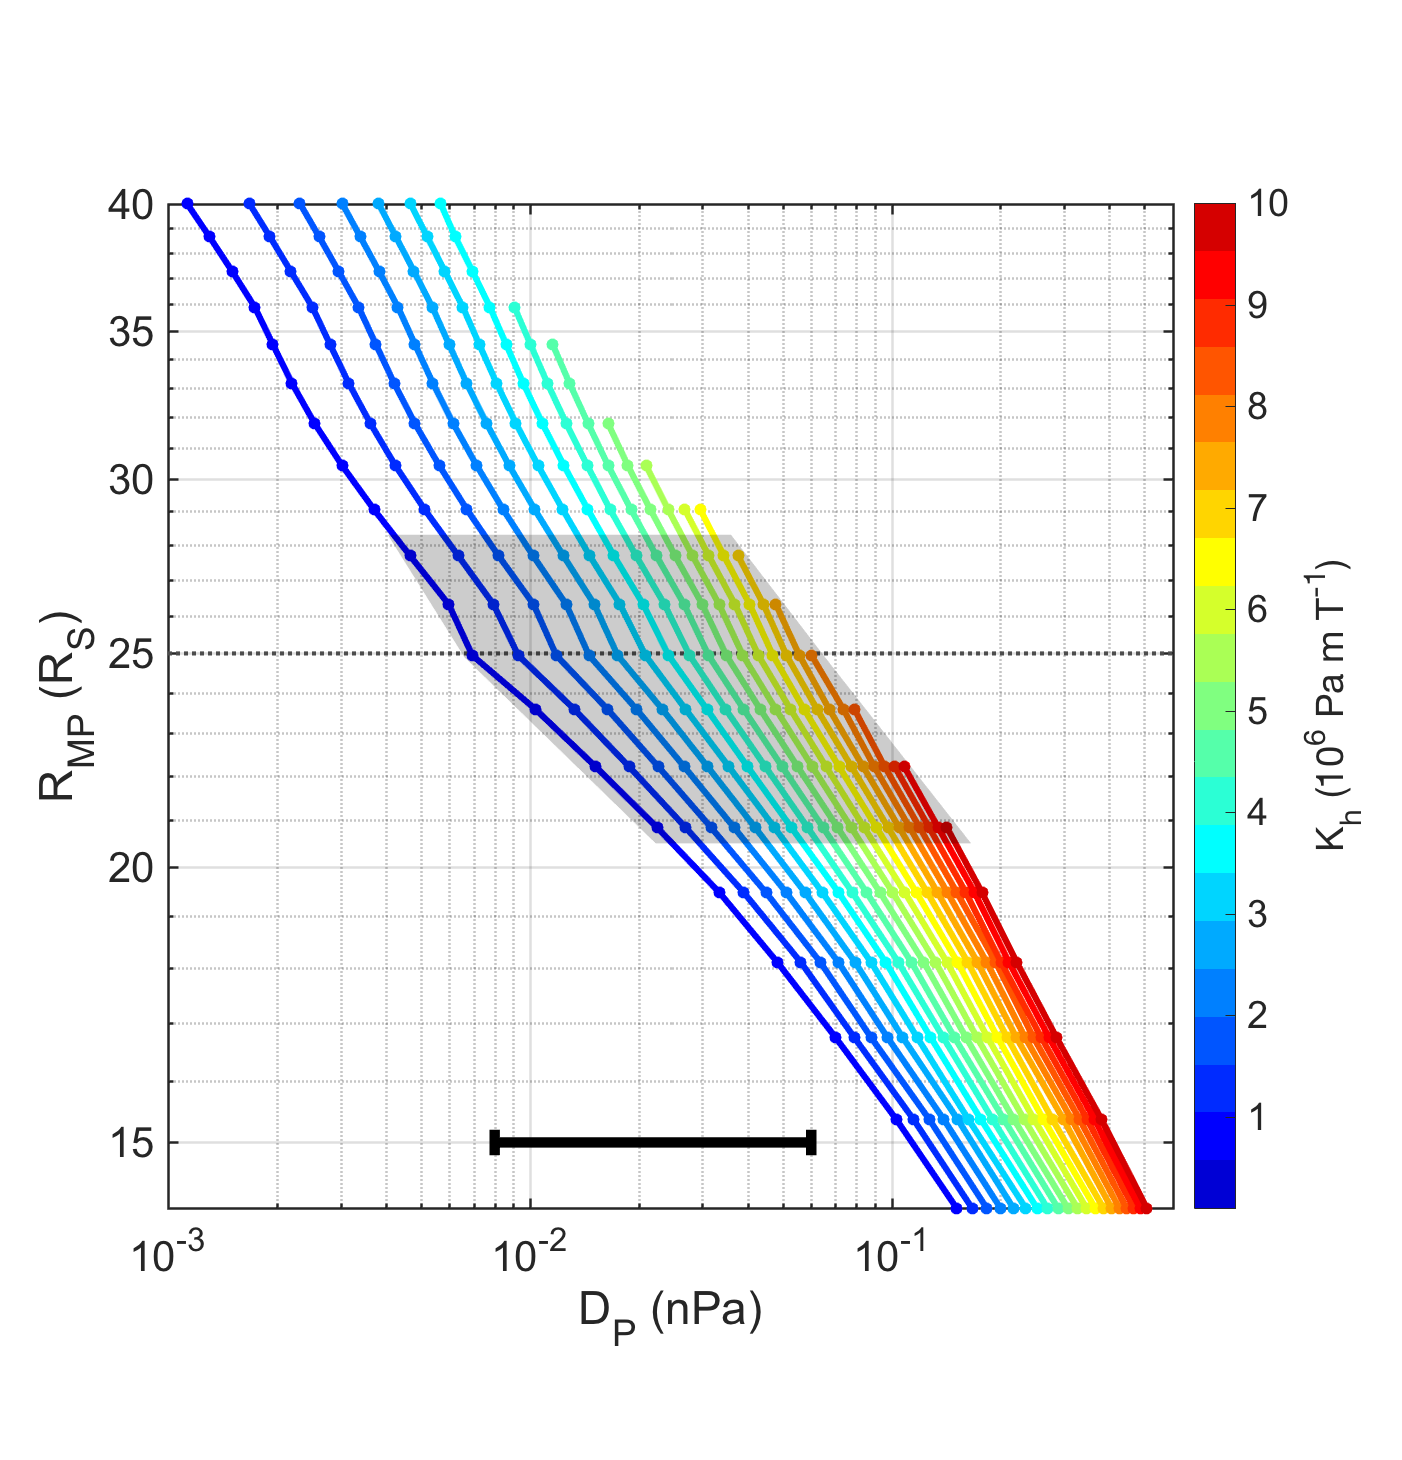
\includegraphics[width=0.8\textwidth]{compress/money2.pdf}
\caption[Magnetopause radius versus solar wind dynamic pressure compressibility profiles for a range of $K_\mathrm{H}$.]{Magnetopause radius $R_\mathrm{MP}$ as a function of solar wind dynamic pressure $D_\mathrm{P}$, on a logarithmic scale, for different $K_\mathrm{H}$ values as shown by the colour bar. Each solid dot represents the result of one model calculation. A dashed line at $R_\mathrm{MP}{=}\SI{25}{R_S}$ is shown for reference. The grey shaded region highlights data points with $R_\mathrm{MP}$ in the range $20.5{\--}\SI{28.3}{R_S}$, corresponding to expected values at Saturn according to empirical observations by \citet{achilleos2008}. The black horizontal bar shows the approximate range of $D_\mathrm{P}$ typically observed at Saturn ($0.008 {\--} \SI{0.06}{nPa}$) according to \textit{Cassini} CAPS solar wind data, also from \citet{achilleos2008}. However it should be noted that values of $D_\mathrm{P}$ in the full range shown in this figure ($0.001 {\--} \SI{0.5}{nPa}$) have been observed empirically.} 
\label{compress:fig:money2}
\end{figure}
 
For sufficiently high values of the hot plasma index, the model calculation would not converge to the prescribed 0.5$\%$ tolerance for large magnetopause radii, hence the lack of coverage in this region of parameter space. We attempted to mitigate this by, at each iteration, weighting the previous Euler potential solution $\alpha_{i-1}(r,\mu)$ up to 10 times more heavily than $\alpha_{i}(r,\mu)$ (see Section \ref{intro:sec:forcebalancemodel}), such that it would approach a convergent solution more slowly. However the correspondingly more stringent tolerance required in this case was still not achieved. The reason for this lack of convergence is that in such circumstances an equilibrium force-balance solution cannot be found, for a field structure that can contain such a level of simulated hot plasma. It is interesting to note that this only occurs under physical conditions we would not expect to typically observe the magnetosphere; for typical values of hot plasma content and solar wind dynamic pressure observed at Saturn, the model calculations are well within the convergence limit, as shown by the black horizontal bar in Figure \ref{compress:fig:money2}.

The most obvious feature apparent in Figure~\ref{compress:fig:money2} is the effect of the hot plasma content on the parameter $a_1$, reflected in the shift of the y-intercept for different compressibility profiles. Estimates of this parameter vary from $10.1 \pm 0.2$ for $K_\mathrm{H}=\SI{1e5}{\pascal\meter\per\tesla}$ to $11.3 \pm 0.03$ for $K_\mathrm{H}=\SI{1e7}{\pascal\meter\per\tesla}$, measured by applying a linear least squares regression line to the entire profile for each $K_\mathrm{H}$ value. This is comparable to the behaviour observed empirically by \citet{pilkington2015} (discussed in Section~\ref{compress:sec:prevstudies}), who calculated that their estimates of $a_1$ varied from ${\sim}11$ for the data set grouped by low average plasma $\beta$ ($\beta\lesssim 1$), to ${\sim}16$ for the data set with high average $\beta$ ($\beta\gtrsim 10$). However it should be noted that, while positively correlated, global hot plasma content $K_\mathrm{H}$ and local plasma $\beta$ are not interchangeable concepts, and have a relationship that is dependent on magnetosphere size, as discussed in detail later. 

These observations of variable $a_1$ correspond to the magnetosphere being observed in a range of sizes for fixed solar wind dynamic pressure, up to $10{\--}\SI{15}{R_S}$ in both \citet{pilkington2015} and this study. \citet{pilkington2015} interpreted this observation theoretically as the magnetosphere existing in either a plasma-depleted or plasma-loaded state, transitioning between these states perhaps via Vasyliunas-style reconnection and associated ejection of plasmoids \citep{vasyliunas1983}, or interchange events \citep{mitchell2015}. If we assume that such transitions can occur at least to some degree independently of the incident solar wind dynamic pressure, then it seems intuitive that there should exist a range of possible system sizes for a fixed $D_\mathrm{P}$, but different $K_\mathrm{H}$. 

This can be explained as follows. Consider a magnetopause initially in dynamic equilibrium with the upstream solar wind dynamic pressure, and what happens when the plasma pressure inside the magnetopause boundary drops due to some plasma loss process. The pressure across the boundary is now unbalanced, with the incident $D_\mathrm{P}$ greater than the total plasma and magnetic pressure inside the magnetosphere. The magnetopause location therefore moves inwards and the magnetosphere is compressed, causing an enhancement in the magnetic field strength $B$. The magnetic pressure therefore increases inside the magnetopause boundary, until pressure balance is restored and a new equilibrium magnetopause location is found. We would also expect the remaining magnetospheric plasma pressure to in general increase as the magnetopause moves inwards. This scenario thus corresponds to the magnetosphere generally being observed at a smaller size when the plasma content or pressure is lower, resulting in a lower estimate for the parameter $a_1$.

The variation in compressibility behaviour with varying system size and hot plasma content shown in Figure~\ref{compress:fig:money2} is less intuitive. As with our initial results, there appears to be a shift in behaviour at around $\SI{25}{R_S}$ for all profiles, although becoming less pronounced as $K_\mathrm{H}$ increases. Therefore for each individual profile at a given $K_\mathrm{H}$ value, the simulated data were again divided into two groups, a compressed regime and an expanded regime, separated at $\SI{25}{R_S}$, and we applied linear fits to these regions separately to make estimates of $\alpha$. The resulting estimates are shown in Figure~\ref{compress:fig:alphas}. Groups with fewer than three individual data points were not fit, hence for the expanded regime the estimates do not cover the full range of $K_\mathrm{H}$.
\begin{figure}
\centering
\noindent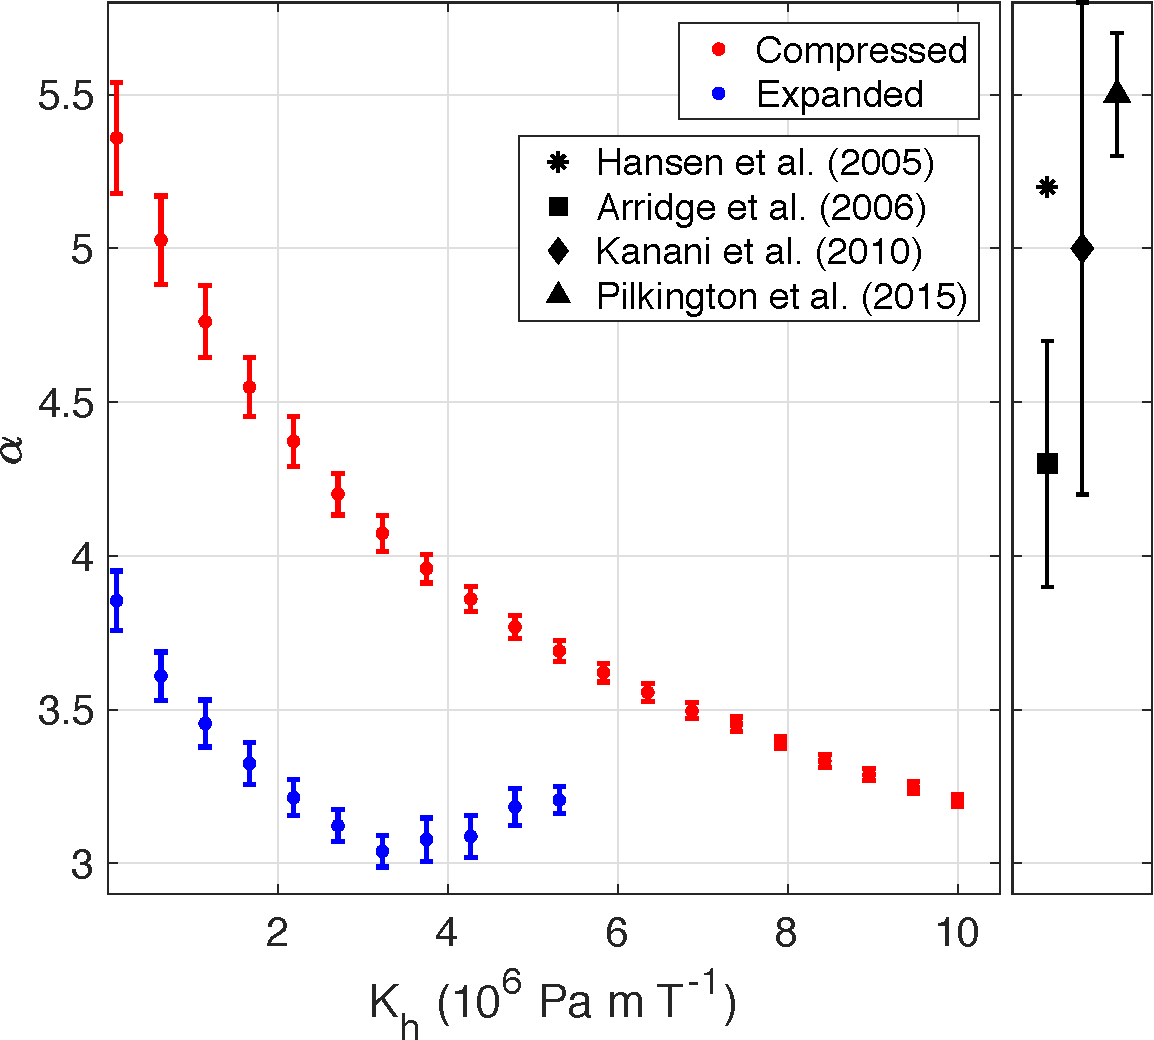
\includegraphics[width=0.8\textwidth]{compress/alphas.pdf}
\caption[Estimates of magnetospheric compressibility parameter $\alpha$, for different system sizes and $K_\mathrm{H}$ values.]{Left panel: estimates in the compressibility parameter $\alpha$, as a function of hot plasma index $K_\mathrm{H}$. Estimates made using the compressed regime profiles ($R_\mathrm{MP} \leq \SI{25}{R_S}$) are shown in red, and those for expanded regime profiles ($R_\mathrm{MP} > \SI{25}{R_S}$) are shown in blue, with error bars corresponding to the standard error in estimated parameters (see Appendix). Right panel: previous results from the literature with uncertainties as described in Table~\ref{compress:table:prevstudies}, included for comparison. Note that in this panel only the $x$ axis does not correspond to any physical quantity.}
\label{compress:fig:alphas}
\end{figure}

As with the initial results, it can be seen that across the full range of $K_\mathrm{H}$, the expanded regime gives lower estimates of $\alpha$ than the compressed regime, corresponding to a magnetosphere that is more sensitive to changes in solar wind pressure as it expands. We suggested in the previous section that this was due to the formation of a significant magnetodisc structure, which is more easily compressible than a dipolar magnetic field structure, only for an expanded magnetosphere. It is also apparent in Figure~\ref{compress:fig:alphas} that there is a general trend of $\alpha$ decreasing as hot plasma content increases, corresponding to a more easily compressible magnetosphere. (Note that for $K_\mathrm{H} > \SI{4e6}{\pascal\meter\per\tesla}$ for the expanded regime, results may be affected by applying a linear fit to so few data points.) \citet{achilleos2010b} found in a previous study using this same model that an increase in hot plasma content did significantly affect the magnetic field configuration, causing a more disc-like field structure, and demonstrated there was reasonable agreement with limited \textit{Cassini} observations. Therefore a similar argument as to how the compressibility changes as the magnetosphere expands, can be employed to explain how the compressibility changes as $K_\mathrm{H}$ increases. This effect can be interpreted as the increased hot plasma pressure augmenting the azimuthal ring current in the magnetosphere, which in turn enhances the associated disc-like magnetic field.

However this is not the full picture. Figure \ref{compress:fig:hotbetacontour} shows a contour plot of how the value of $\beta_\mathrm{H}$ at the nose of the magnetosphere, just inside the magnetopause boundary, varies with both magnetopause radius and hot plasma index. Values are extracted from all models where convergence was obtained. For the initial conditions described in this study, $K_\mathrm{H}=\SI{1e6}{\pascal\meter\per\tesla}$, we found that $\beta_\mathrm{H}$ never exceeded ${\sim}0.7$ for any system size, and thus the variation in magnetic pressure with radial distance always controlled the compressibility behaviour. However we can see that in the extremes of allowed parameter space, where either $K_\mathrm{H}$ or $R_\mathrm{MP}$ are sufficiently large, $\beta_\mathrm{H} > 1$ and therefore the variation in hot plasma pressure with radial distance also becomes important in controlling the compressibility behaviour. These conditions correspond directly to regions where $\alpha$ is lower, suggesting that a sufficiently high hot plasma pressure makes the magnetosphere more easily compressible. For values of $K_\mathrm{H}$ near the upper limits of empirical observations, approaching $10^7~\si{\pascal\meter\per\tesla}$, it can be seen in Figure~\ref{compress:fig:hotbetacontour} that $\beta$ exceeds unity even for the smallest system sizes, and indeed it is in this region of parameter space that the smallest estimates of $\alpha$ are obtained. However, it was found by \citet{pilkington2015} that such conditions of a compressed magnetosphere with high hot plasma content, were rarely observed empirically, which may partially explain the discrepancy between previous results and our lowest $\alpha$ estimates, shown in Figure~\ref{compress:fig:alphas}. This can also be seen in Figure~\ref{compress:fig:money2}, which shows that the solar wind dynamic pressure typically observed at Saturn is not sufficiently high to support such compressed magnetospheres with high hot plasma content. (Note that cold plasma beta $\beta_\mathrm{C}$ was never found to exceed 0.7 anywhere in the allowed parameter space and thus is not discussed further.)
\begin{figure}
\centering
\noindent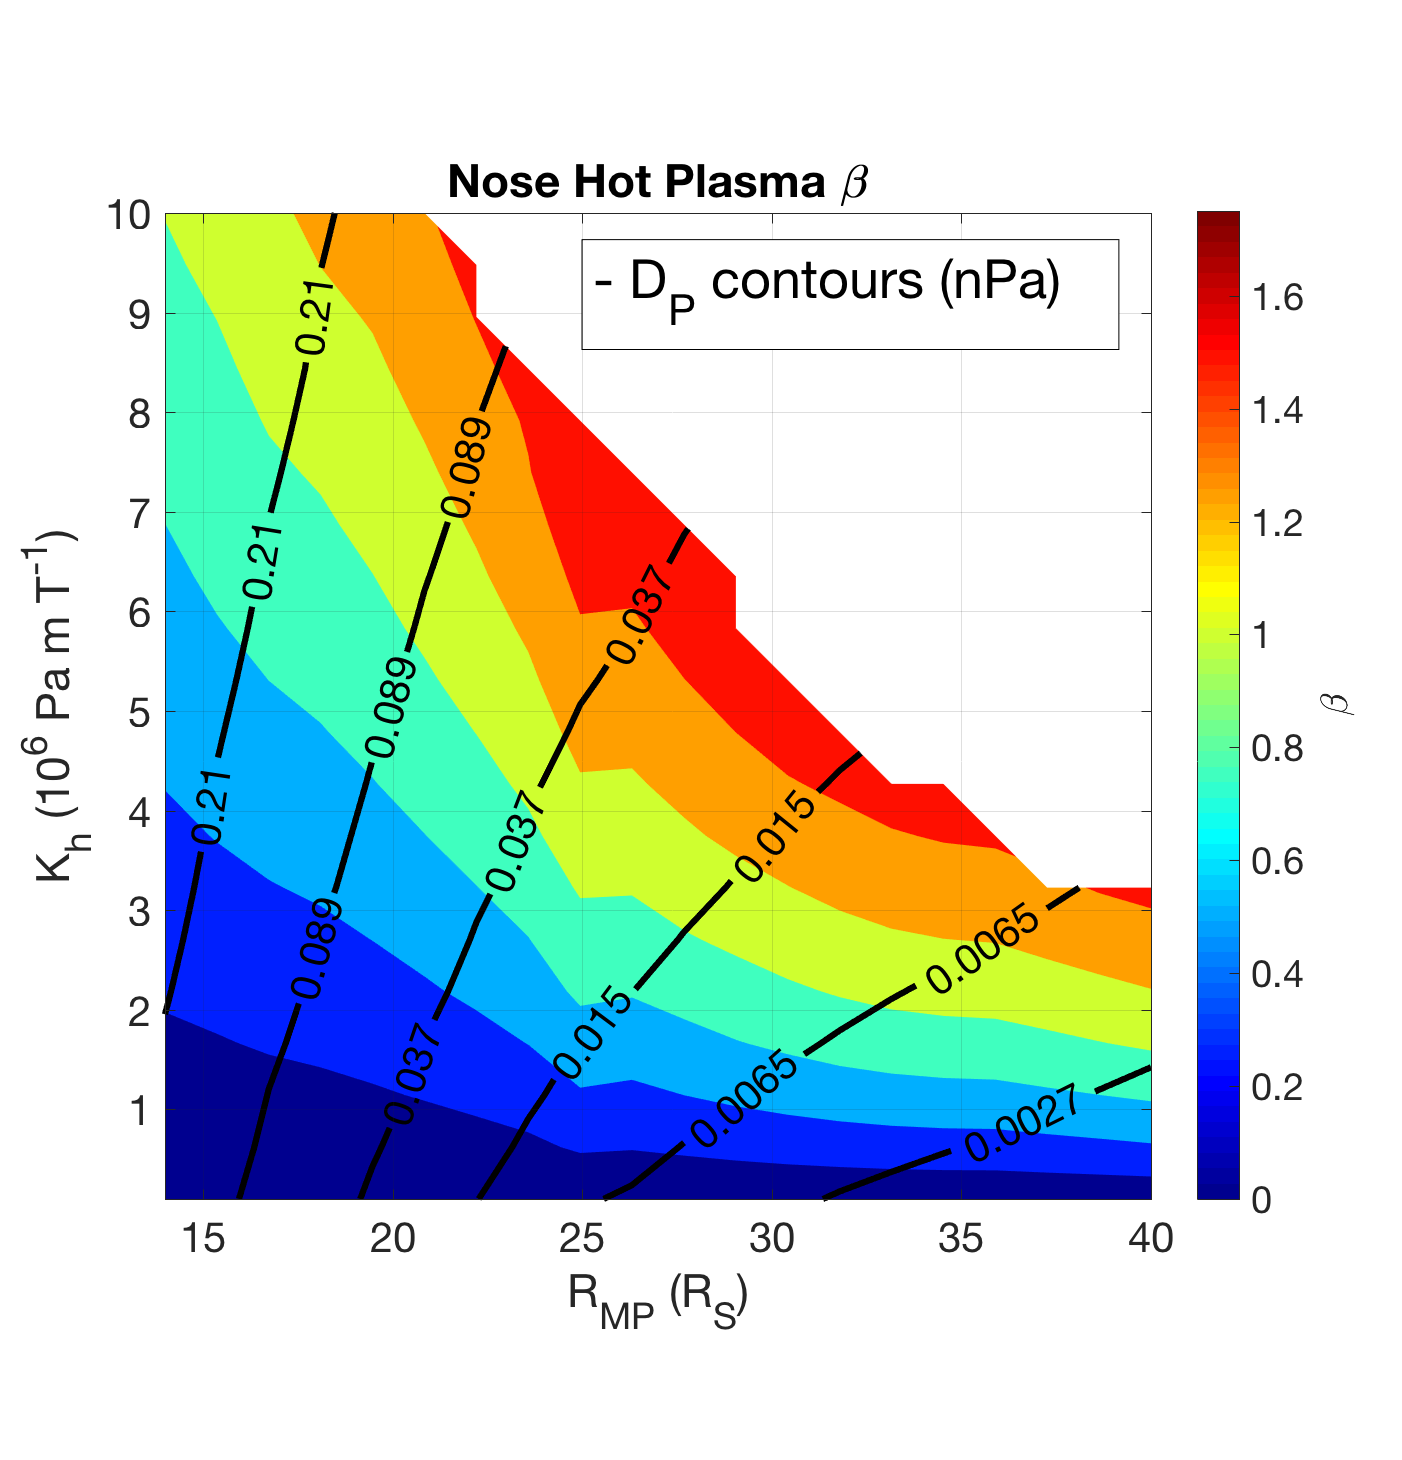
\includegraphics[width=0.7\textwidth]{compress/hotbetacontour.pdf}
\caption[Map of hot plasma $\beta$ just inside the magnetopause boundary in system size, $K_\mathrm{H}$ parameter space.]{Hot plasma $\beta$ at the nose of the magnetosphere just inside the magnetopause boundary, varying with both magnetopause radius $R_\mathrm{MP}$ and hot plasma index $K_\mathrm{H}$. The $\beta$ value is indicated on a colour scale. Contours of constant solar wind dynamic pressure $D_\mathrm{P}$ are shown as black lines, labelled with values in units of nPa.}
\label{compress:fig:hotbetacontour}
\end{figure}

For a dipolar magnetic field with isothermal plasma transport, it was explained in the introduction that we would expect $P_\mathrm{H} \propto r^{-4}$, thus giving $\alpha \approx 4$ for a magnetosphere with compressibility controlled by hot plasma content. However Figure \ref{compress:fig:alphas} shows we find $\alpha < 4$ in the most extreme cases. Indeed, when fitting the profiles of hot plasma pressure specifically for each $K_\mathrm{H}$ value, it was found that for these model calculations, the behaviour varied from $P_\mathrm{H} \propto r^{-3.3}$ for the smallest hot plasma index to $\propto r^{-2.6}$ for the greatest, corresponding to a reduction in compressibility parameter $\alpha$. It was also found that, unlike the magnetic pressure profiles, there was no considerable shift in behaviour at $\SI{25}{R_S}$, and so the observed kink in Figure \ref{compress:fig:hotbetacontour} in this region is solely due to change in magnetic pressure, the denominator of $\beta_\mathrm{H}$.

This behaviour of the hot plasma pressure can be further understood as follows. The parameterisation of hot plasma adopted in this model means that $P_\mathrm{H}$ is fully determined by how the flux tube volume varies with system size, as $P_\mathrm{H}V=K_\mathrm{H}$. The flux tube volume is defined in equation (\ref{compress:eq:ftv}), and is thus dependent on both the length of a given field line ($ds$) and the magnetic field strength ($B$). For a dipolar field line, $B \propto r^{-3}$ and $\int ds \propto r$, hence $V \propto r^4$ and $P_\mathrm{H} \propto r^{-4}$ in our parameterisation. However in this model, as we have discussed, we have found that the magnetic field strength varies more slowly with radial distance than this, particularly in expanded regimes and with high hot plasma content. Indeed the behaviour varies from $B \propto r^{-2.7}$ for compressed regimes with low hot plasma content, to $\propto r^{-1.8}$ for expanded regimes with high hot plasma content, corresponding to a more significant magnetodisc field. This in turn affects how flux tube volume varies with system size, meaning $P_\mathrm{H}$ varies more slowly with system size.

In addition, we also observed that for more expanded systems, the length of the outermost magnetic field lines $\int ds$ varied more slowly with radial distance than for a dipolar magnetic field, with $\int ds \propto r^{0.9}$ for magnetospheres with the lowest $K_\mathrm{H}$ values, to $\propto r^{0.8}$ for the highest $K_\mathrm{H}$ values. For more expanded, stretched magnetospheres, it is perhaps intuitive that the magnetic field lines in the outer regions have shorter overall lengths than a corresponding dipolar magnetic field line that crosses the equator at the same radial distance, due to the outward radial stretching of the dipole magnetic field associated with the ring current. Figure \ref{compress:fig:LCFL} illustrates this oblateness of the magnetospheric magnetic field lines observed in our model calculations, and how it increases with system size and hot plasma content. Each panel illustrates how the shape of the outermost closed magnetic field line, which crosses the equator at the magnetopause nose, varies with the size of the magnetosphere, for a given $K_\mathrm{H}$ value. The shape is shown in height above the rotational equator $Z$ and cylindrical radial distance from the planet centre $\rho$, normalized to the magnetopause radius $R_\mathrm{MP}$, with a representative dipolar magnetic field line shown in black on each plot for comparison.
\begin{figure}
\centering
\noindent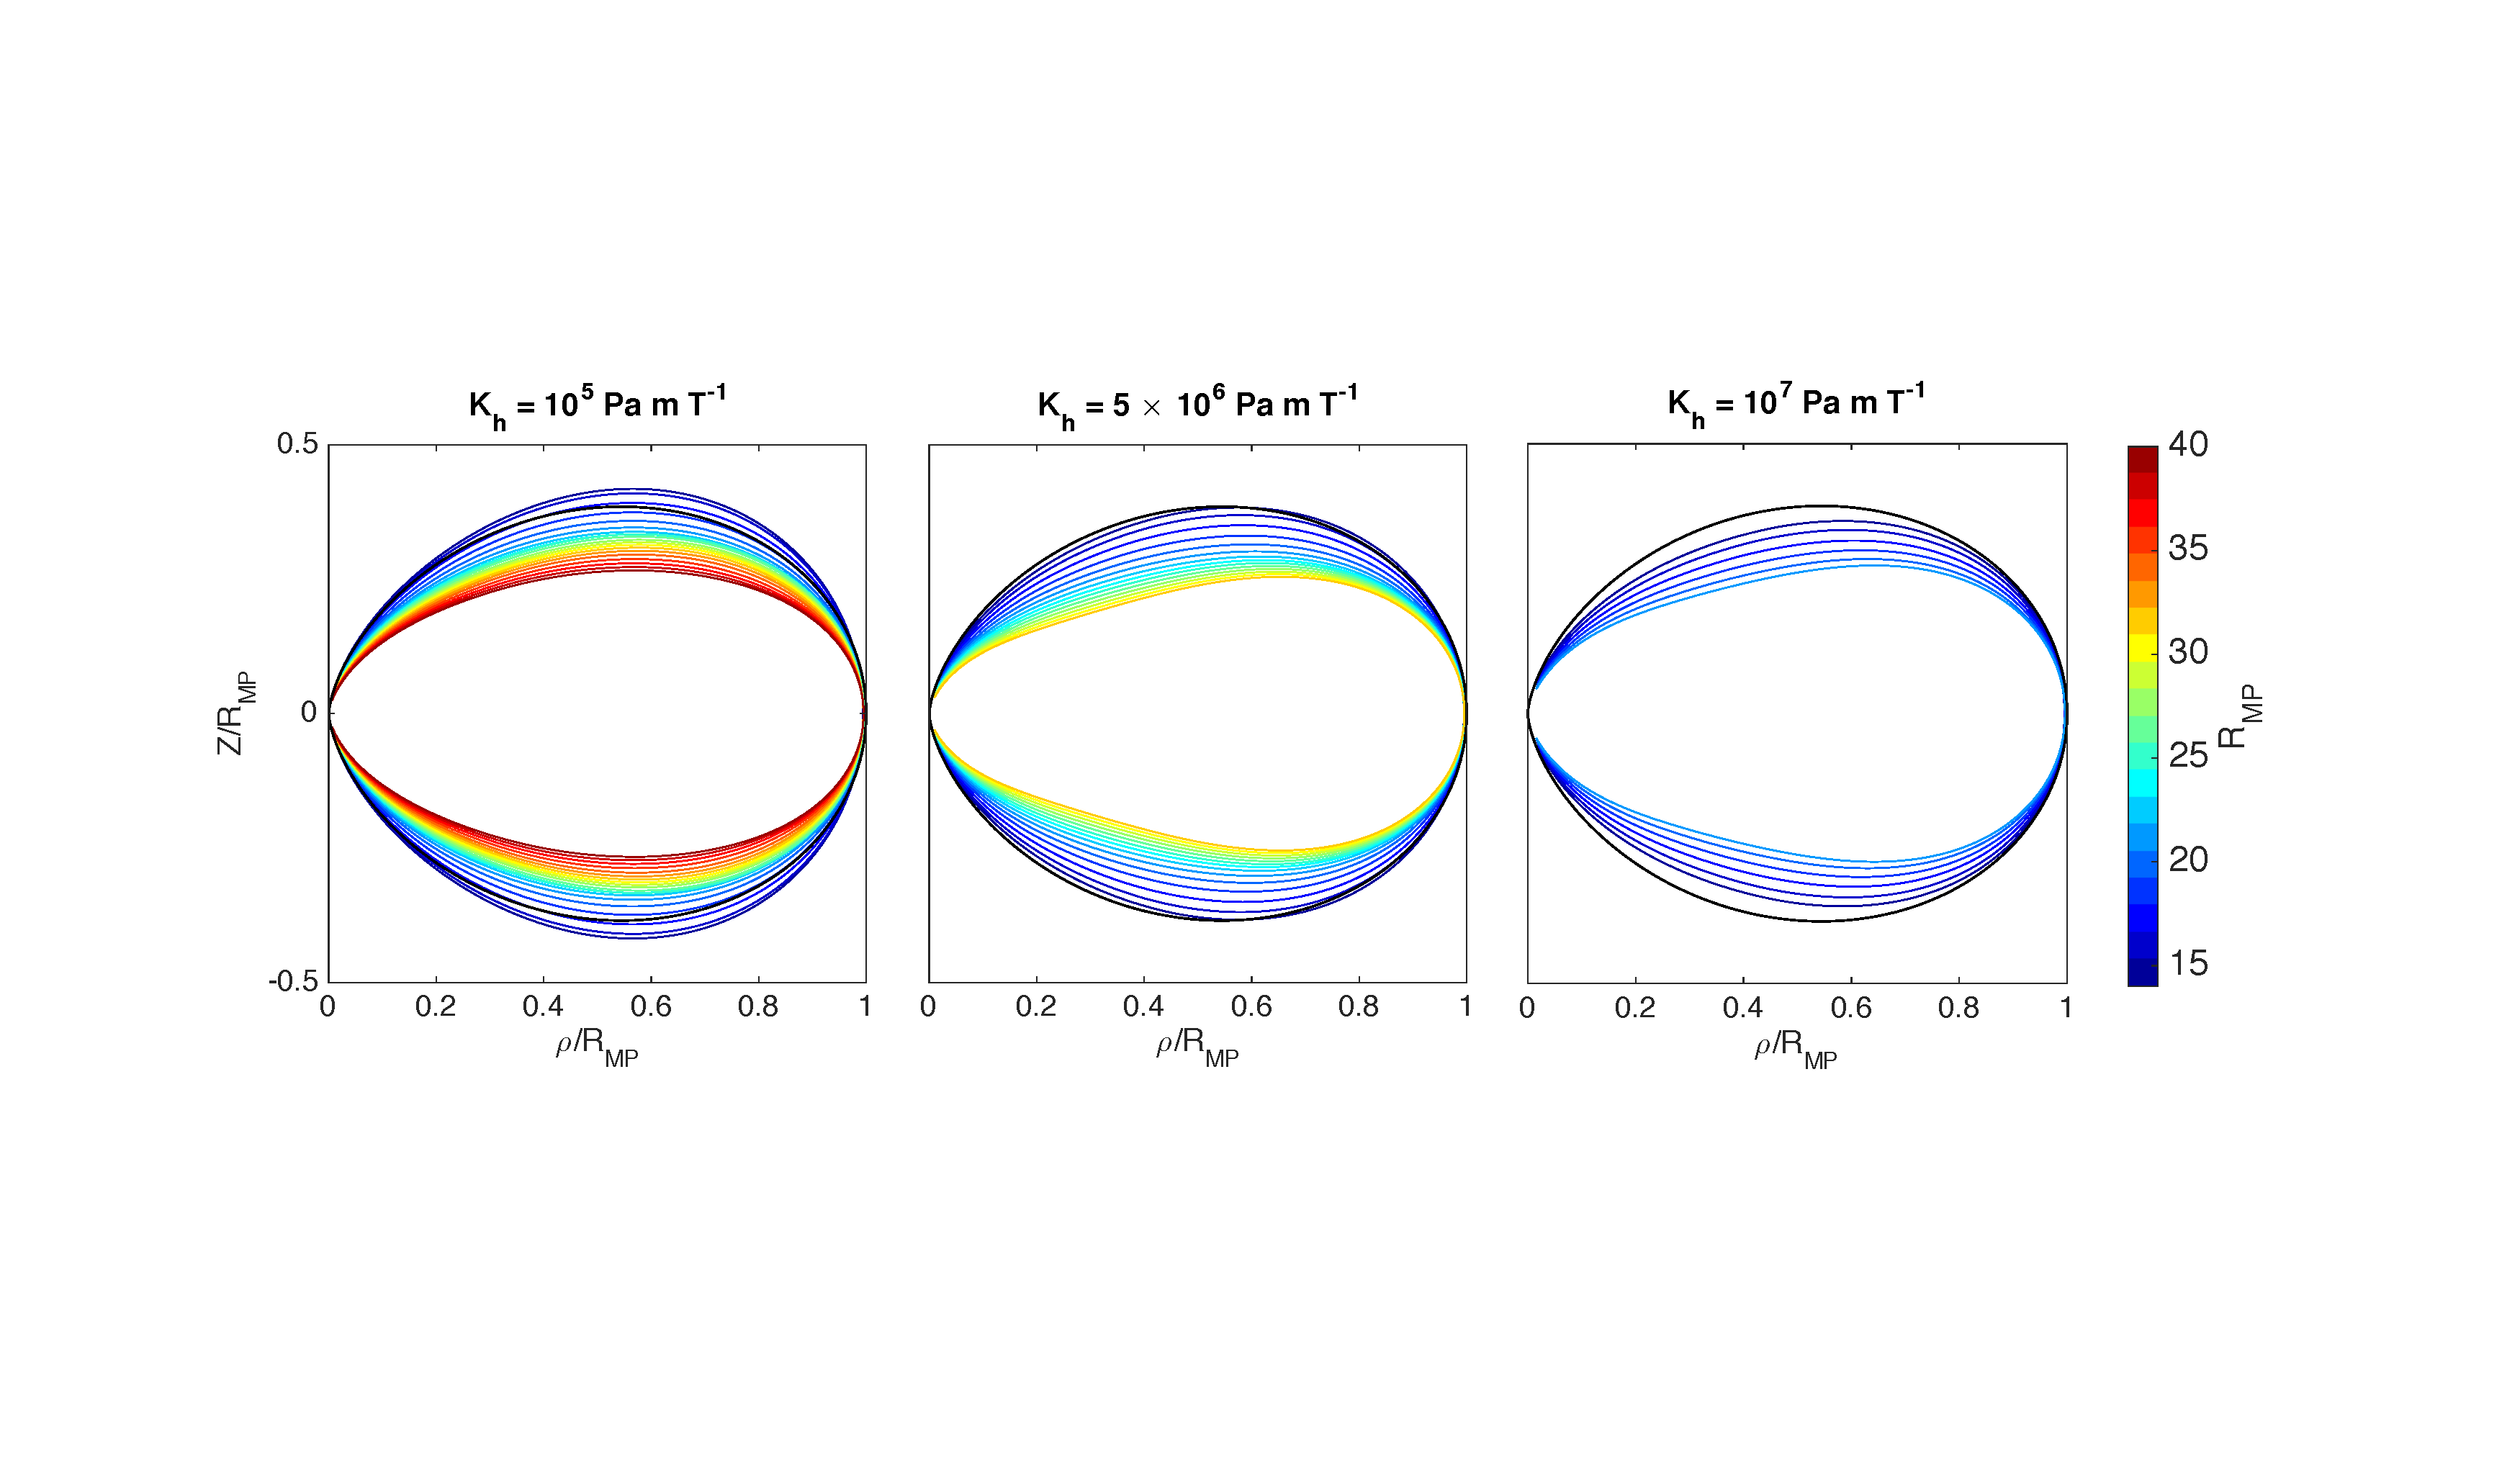
\includegraphics[width=\textwidth]{compress/LCFL.pdf}
\caption[Outermost magnetic field line shapes for the range in system size, $K_\mathrm{H}$ parameter space.]{The shape of the outermost closed field line in a magnetosphere as the magnetopause radius $R_\mathrm{MP}$ changes, for three different values of $K_\mathrm{H}$ corresponding to very quiet, average and disturbed ring currents respectively. In each panel the shape of the field line has been normalized in the vertical and horizontal direction by the magnetopause radius $R_\mathrm{MP}$, the value of which is shown by the colour of the field line according to the colour bar. A representative dipolar magnetic field line is shown in black on each plot for comparison.}
\label{compress:fig:LCFL}
\end{figure}

It can be seen clearly that as the magnetosphere size increases the outermost closed field line is confined comparatively much more towards the equator than for the magnetospheres with smaller $R_\mathrm{MP}$. This is especially pronounced for the magnetospheres with higher hot plasma content, where the field lines show significant oblateness particularly at lower $\rho$. 

This effect can be interpreted theoretically as follows. Considering pressure balance perpendicular to a magnetic field line in the outer magnetosphere, the two dominant forces to consider are the hot plasma pressure gradient and the centrifugal force. The force associated with the plasma pressure gradient acts outwards from the center of curvature of the field line, perpendicular to the field line, across the entire field line length. This property arises as a consequence of plasma pressure being assumed constant along a field line (see Section \ref{compress:sec:model}). In contrast, the centrifugal force acts in the direction of increasing $\rho$. Therefore the component of centrifugal force perpendicular to the magnetic field line can either act outwards away from or inwards towards the equatorial plane depending on the geometry, acting inwards for smaller $\rho$, and outwards beyond the `turning' point of the magnetic field line, when the field line begins to converge back towards the equator. This turning point occurs about half away along the magnetosphere, at around 0.5 $\rho/R_\mathrm{MP}$, for the compressed, low $K_\mathrm{H}$ cases, but as far out as 0.7 $\rho/R_\mathrm{MP}$ for the most expanded and hottest cases. The further out in radial distance that this turning point occurs, the higher the fraction of the magnetic field line for which the perpendicular component of centrifugal force is acting inwards, towards the equatorial plane - and thus effectively balancing the outwards hot plasma pressure gradient force. Therefore in order to maintain global force balance, this turning point moves radially outwards as the hot plasma pressure gradient increases, and the field line thus becomes more confined.

We explained in Section~\ref{compress:sec:model} that the parameterisation of hot plasma content via the state equation involving the index $K_\mathrm{H}=P_\mathrm{H}V$ was a simplifying assumption in light of variable observations of hot plasma pressure. However it would have also been possible to instead parameterise the hot plasma content by, for example, $K_\mathrm{H}=P_\mathrm{H}V^\gamma$, with $\gamma=5/3$, such that magnetic flux tubes of plasma are considered to expand and contract adiabatically rather than isothermally. The factors of $B$ and $\int ds$ that determine the flux tube volume $V$ would be unchanged, however the previous relationship $P_\mathrm{H}\propto V^{-1}$ would be modified to $P_\mathrm{H} \propto V^{-\gamma}$. For a magnetosphere with compressibility controlled by hot plasma content, this corresponds to an increase in the estimate of the compressibility parameter $\alpha$ by a factor of $\gamma$, and thus a magnetosphere that is less sensitive to changes in solar wind dynamic pressure. This aspect may also contribute to the discrepancy between our results and those of previous empirical studies, shown in Figure~\ref{compress:fig:alphas}, as the plasma population may behave intermediately between the two state equations discussed in this study. Indeed, the analysis of \citet{achilleos2010a} supports this conclusion.

\subsection{Comparison with the Jovian System}\label{compress:sec:jup}
It is insightful to make a comparison between the results presented here and the corresponding calculations for Jupiter's magnetosphere, using our implementation of the model of \citet{caudal1986} directly. Figure~\ref{compress:fig:jupmoney} shows the results for Jovian calculations analogous to Figure~\ref{compress:fig:money1} for the Saturn case. Jovian magnetopause radii in the range $R_\mathrm{MP} = 50{\--}\SI{100}{R_J}$ have been used to cover the observed range presented in previous studies \citep{joy2002}.
\begin{figure}
\centering
\noindent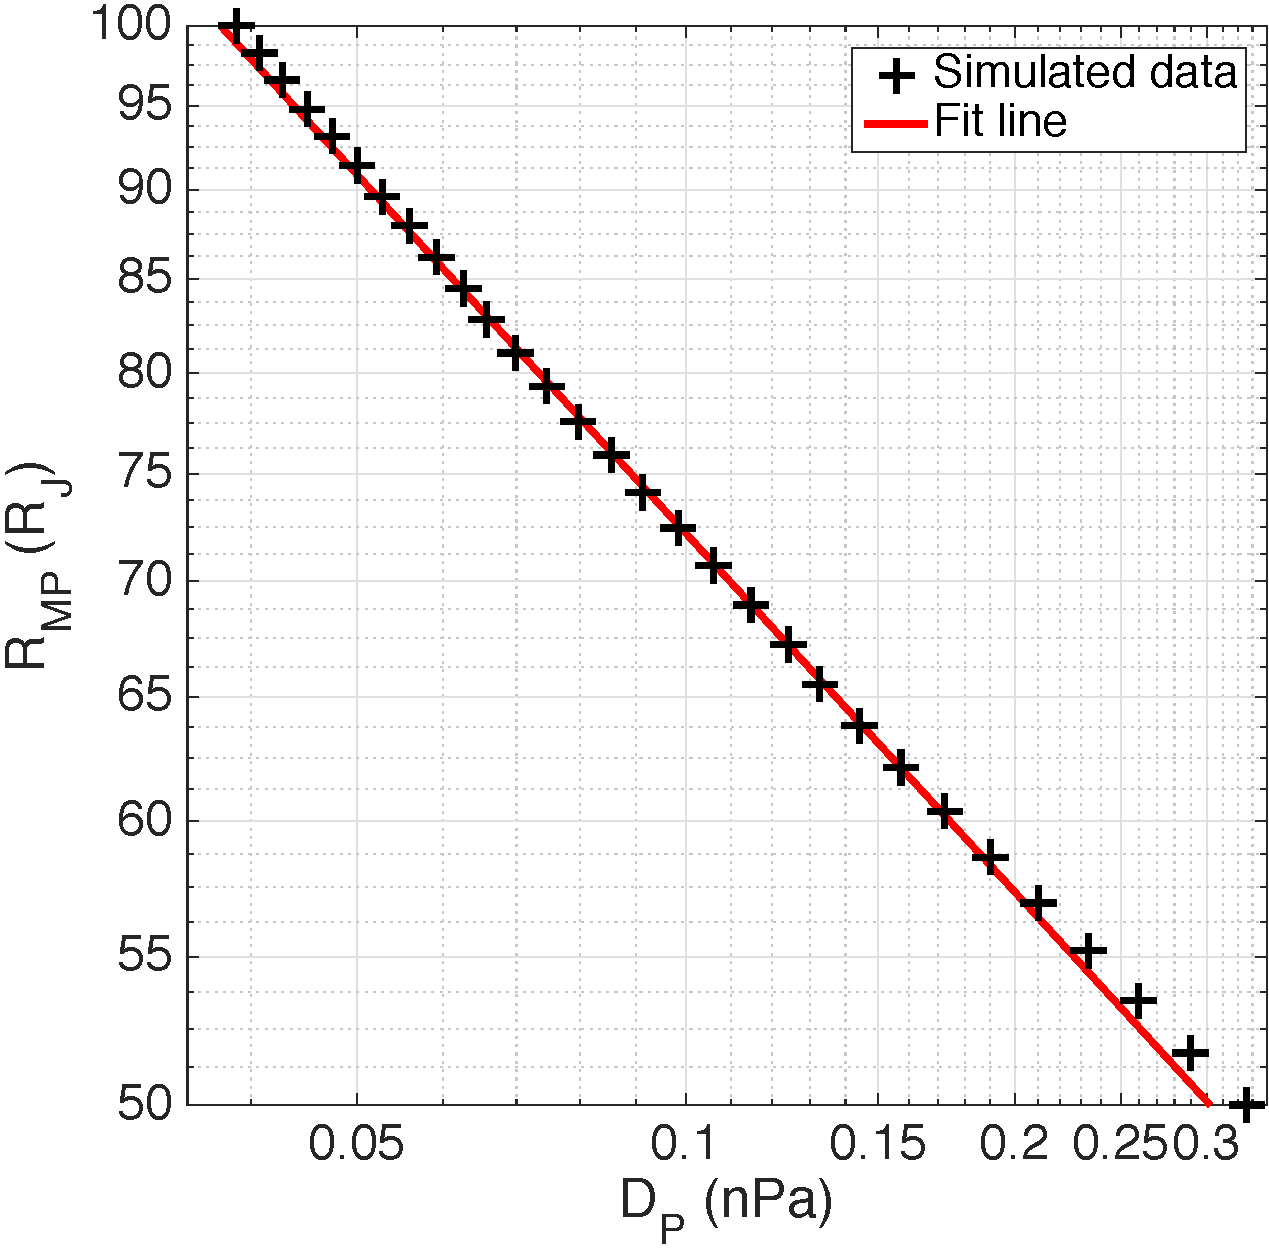
\includegraphics[width=0.7\textwidth]{compress/jupmoney.pdf}
\caption[Magnetopause radius versus solar wind dynamic pressure profile for Jupiter's magnetosphere.]{Magnetopause radius $R_\mathrm{MP}$ as a function of solar wind dynamic pressure $D_{P}$, on a logarithmic scale, for the magnetosphere of \textbf{Jupiter}. Each black cross represents the result of one model calculation. The linear least squares regression line fitted to calculations is shown in red.}
\label{compress:fig:jupmoney}
\end{figure}

It can clearly be seen that, unlike the Saturn case, the Jovian magnetosphere shows a compressibility behaviour that is well represented by a uniform $\alpha$ across all observed system sizes, demonstrated by a constant gradient of the $D_\mathrm{P}$ profile. A single linear least squares regression line fit provided an estimate for the compressibility parameter $\alpha=3.05 \pm 0.02$. As for the Saturn case, the data were split into two groups representing a compressed and expanded regime, and a linear least squares regression line was fit to each group separately. However, this did not provide significantly different estimates for $\alpha$, with a variation of only approximately 6$\%$ between groups, and so only the fitting for the entire simulated data set is shown and discussed here. This value of $\alpha=3.05 \pm 0.02$ is remarkably smaller than observational studies in the literature, which estimate this value as between ${\sim}4$ and ${\sim}5$ \citep{huddleston1998,joy2002,alexeev2005}. Possible reasons for this discrepancy are discussed at the end of this section. However it can be seen from a comparison with Figure \ref{compress:fig:alphas} that this value is consistent with our original theoretical expectation that this value be lower than that of the Saturn system, due to arguments discussed in Section~\ref{compress:sec:intro}.

It is worth noting that this difference in behaviour between the Saturnian and Jovian magnetospheres is also a consequence of their relative locations in the solar system, and the weaker solar wind dynamic pressure experienced at Saturn. If Saturn were to be located closer to the Sun such that it experienced the higher solar wind dynamic pressures typically observed at Jupiter, then the Saturnian magnetosphere would also show a compressibility behaviour represented by a uniform $\alpha$, specifically corresponding to its compressed regime. This can be seen by comparing the ranges in solar wind dynamic pressure in Figure \ref{compress:fig:money1} and Figure \ref{compress:fig:jupmoney}.

We compared the individual $P_\mathrm{H}$, $P_\mathrm{C}$ and $P_\mathrm{B}$ components that comprise the $D_\mathrm{P}$ estimate across all system sizes and found that, as with the initial results for the Saturn case presented in Figure~\ref{compress:fig:pcomps}, the magnetic pressure component was dominant across all system sizes. Both hot and cold plasma $\beta$ monotonically increased with system size, with $\beta_\mathrm{C} \leq 0.3$ and $\beta_\mathrm{H} \leq 0.8$ across the simulated data set. Unlike the Saturn case, there was no evidence of a shift in gradient of the magnetic pressure ($P_\mathrm{B}$) profile for increased values of $R_\mathrm{MP}$; we measured a constant slope equivalent to $P_\mathrm{B}\propto r^{-3.4}$, corresponding to $B\propto r^{-1.7}$. This index is smaller than was measured even in the hottest and largest magnetosphere models in our Saturn investigation, and corresponds to a very significant disc-like distortion from a dipolar magnetic field for all Jupiter $R_\mathrm{MP}$. Comparable behaviour is expected theoretically as discussed in Section~\ref{intro:sec:comparativemagnetospheres} of this thesis, and has also been observed empirically \cite[e.g.][]{khurana1989}. We also found that the hot plasma pressure $P_\mathrm{H}$ varied as $P_\mathrm{H} \propto r^{-2.7}$, comparable to the behaviour measured for the hottest and largest magnetosphere models in our Saturn investigation. This can readily be explained via the same arguments applied to the Saturn case in the previous section.

As with our initial Saturn investigation, we estimated the pressure contribution from the centrifugal force at the magnetopause boundary, using a very approximate value for the magnetopause boundary layer thickness of $\SI{1}{R_J}$ following \citet{delamere2010}. We found that the centrifugal term was at least an order of magnitude smaller than all other pressure components at the magnetopause boundary across all system sizes, and therefore does not play a significant role in determining compressibility. However in a study by \citet{nichols2011}, it was suggested that this Jovian model may significantly underestimate the magnitude of centrifugal force in the middle and outer magnetosphere, due to the use of a plasma angular velocity profile that overestimates the breakdown of corotation. This would mean that the model would also overestimate how strongly the centrifugal force falls with radial distance. In combination, these effects may contribute to the discrepancy between our particularly low estimate of the compressibility parameter $\alpha$ for the Jovian magnetosphere, and previous empirical studies. While beyond the scope of the  current work,  it  would be insightful to investigate this aspect further in future studies, as well as the influence of different hot plasma parameterisations, using more recent spacecraft data sets than the Voyager results employed in the \citet{caudal1986} model.

\section{Summary and Conclusions}
We have employed the UCL/AGA force-balance model of Saturn's dayside magnetosphere, first described in \citet{achilleos2010a}, to investigate magnetospheric compressibility, and in particular its response to solar wind conditions and global hot plasma content. We have found that, for `average' global hot plasma conditions, the compressibility behaviour can be described by equation~\ref{compress:eq:key} but with a value of compressibility parameter $\alpha$ that decreases with system size, from ${\sim}4.8$ for $R_\mathrm{MP} \leq \SI{25}{R_S}$ to ${\sim}3.5$ for $R_\mathrm{MP} > \SI{25}{R_S}$. This corresponds to the magnetosphere becoming more easily compressible as the upstream solar wind dynamic pressure decreases. We have explained this in terms of the distortion of the magnetic field into a magnetodisc configuration, which is more easily compressible than a dipolar magnetic field, and that this distortion becomes significant for more expanded magnetospheres. 

We have shown that the global hot plasma content of the magnetosphere, parameterised by the hot plasma index $K_\mathrm{H}=P_\mathrm{H}V$, also plays an important role in determining magnetospheric compressibility. When Saturn's magnetosphere is compressed, a higher value of $K_\mathrm{H}$ acts to increase the observed magnetospheric compressibility via an enhancement of the aforementioned magnetodisc magnetic field structure, due to its contribution to the associated ring current magnetic field. When the magnetosphere is more expanded, the hot plasma pressure exceeds the magnetic pressure at the magnetopause boundary such that the variation in hot plasma pressure with radial distance becomes significant in controlling magnetospheric compressibility. We have determined that, as the hot plasma pressure $P_\mathrm{H}$ varies more slowly with radial distance than the magnetic pressure $P_\mathrm{B}$, this corresponds to the magnetosphere becoming more easily compressible under such conditions. We also explored the behaviour of the $P_\mathrm{B}$ and $P_\mathrm{H}$ profiles, and how they are related via the flux tube volume $V$. Our estimates of $\alpha$ are in the range ${~}3.3-5.3$ depending on system size and hot plasma content, with lower estimates corresponding to higher values of both of these parameters. However as we have mentioned, these results are sensitive to our simplifying parameterisation of the hot plasma content, and for example would increase up to a factor of $5/3$ (for regions of parameter space where hot pressure is dominant) if we were instead to parameterise the hot plasma content via $K_\mathrm{H} = P_\mathrm{H}V^\gamma$. 

These results thus suggest that future observational studies of the relationship between $R_\mathrm{MP}$ and $D_\mathrm{P}$ may benefit from the assumption that the compressibility parameter $\alpha$ is not constant across all observations, but varies both with system size and hot plasma content, at comparable levels of significance. In addition, our model analysis demonstrates that centrifugal force at the magnetopause boundary does not contribute significantly to the compressibility of the magnetosphere. On the other hand, \textit{global} centrifugal force is important in determining the global field structure, and thus, compressibility. Improvements are needed in our treatment of the plasma angular velocity profile, in order to make it self-consistent with the changing magnetic field structure so as to further test our initial findings.

The investigation in  this chapter has demonstrated in detail how the magnetic field and plasma structure in the UCL/AGA model varies with internal hot plasma conditions, and with system size. In particular, the result that the magnetospheric magnetic field becomes more disc-like as it expands, is utilised in the study presented in the next chapter. In Chapter~\ref{chap:equinox}, we investigate the periodic `flapping' and `breathing' behaviour of Saturn's equatorial current sheet, introduced in Section~\ref{intro:sec:periodicities}.  This breathing behaviour  corresponds to a periodic thickening and thinning of the current sheet at different Saturn  longitudes, associated with a reconfiguration from a more dipolar to a more disc-like magnetic field; we use a modified version of the UCL/AGA model calculated at different system sizes to represent this periodic variation.